\documentclass[12pt,a4paper,bibliography=totocnumbered]{scrartcl}
\usepackage[utf8]{inputenc}
\usepackage[ngerman]{babel}
%\usepackage[USenglish]{babel}
\usepackage{booktabs}
\linespread{1.25}
\usepackage[T1]{fontenc}
\usepackage{amsmath,amssymb,amstext}
\usepackage{graphicx}
\usepackage{fancyhdr}
\usepackage{titling}
\usepackage{color}
\usepackage{array}
\usepackage{chemmacros}
\usepackage{float}
\usepackage{chemexec}     
\usepackage{chemfig,chemnum}
\usepackage{natbib} 
\usepackage[hyphens,spaces]{url}
\newcolumntype{M}[1]{>{\centering\arraybackslash}m{#1}}
\usepackage{multirow}
% URLs im pdf Dokument hinzufügen
\usepackage{hyperref}
\setlength{\parindent}{0em} 

%\addbibresource{literatur.bib}


\begin{document}
	
	
	%switch off page numbering 
\pagenumbering{gobble}

%\thispagestyle{empty}

\setlength\droptitle {-20.5mm}
\renewcommand{\maketitlehooka}{
	
\includegraphics[width=\linewidth]{{picture/HUlogo.png}}\par\vskip 0.7cm}

\title{\normalsize \textbf{LEBENSWISSENSCHAFTLICHE FAKULTÄT\\ INSTITUT FÜR BIOLOGIE}  \\ \vspace*{1.5cm} \vspace*{15pt}
 \Large \textbf{Protokoll}\\ 
 \large \textbf{Fachkurs: Zell- und Membranbiophysik}\\ \vspace*{1.5cm} 
 Versuch: Excimerenbildung von Pyren in Phospholipidmembranen \\ \vspace*{1.5cm} 
 \normalsize Betreuer: Dr. Thomas Korte, Dr. Peter Müller  \\ \vspace*{2.3cm} 
 Jan Piotraschke (\url{piotrasj@hu-berlin.de}) \\ 
 Katja Frenzel (\url{katjafrenzel@gmx.net})  \\ \vspace*{3.4cm}
 Berlin, der 02. Juli 2020 \vspace*{-4.0cm}  }

\date{}
\bibliographystyle{unsrt}
%\cfoot{\thepage}

\maketitle
\textcolor{white}{}

 %\newpage

	\tableofcontents
% \thispagestyle{empty}
%\pagenumbering{arabic} 
%\setcounter{page}{1}

\newpage
	\pagestyle{headings}
\pagenumbering{arabic} 
\setcounter{page}{1}

\section{Einleitung}
NOTE: Einleitung länger machen -> 1-2 Seiten! \\\\

Der vorliegende Versuch untersucht die konzentrations- bzw. temperaturabhängige Excimerbildung von Pyren in Ei-PC (Eilecithin) und DPPC (Dipalmitoylphosphatidylcholin) Vesikeln.\\
Anschließend werden die verschiedenen Lateraldiffusionskoeffizienten von Pyren errechnet. \\

NOTE: Pyren (seine Besonderheiten: etc.etc. ) ermölgicht eine Excimerenbildung basierend auf den Grundalgen ... ...
\\\\
Der Versuch benutzt die Methode der Fluoreszenzmessung. Fluoreszenz kann i.a. bei einem delokalisierten $\pi$-System auftreten, indem ein Chromophor durch die elektrische Komponente einer elektromagnetischen Strahlung vom $S_0$ Grundenergiezustand ausgehend angeregt wird und nach einer gewissen Zeit der $S_1$ Zustand sich mit Strahlung wieder auf den Grundzustand relaxiert.

	\section{Material und Methoden}
Eine detaillierte Beschreibung der Grundlagen, Aufgabenstellung und Versuchsdurchführung ist dem Skript \cite{Kursskript} zu entnehmen. \\

NOTE: Beschreibung der Grundlagen aus dem Skript einfach übernehmen, so der Doktor

Die Messungen der Temperaturabhängigkeit der Excimerenbildung von Pyren in DPPC mit Cholesterol (siehe Skript Teil B (iii)) wurde nicht gemacht.


\newpage
	\section{Ergebnisse}
\subsection{Anregungs- und Emissionspektrum von Pyren}
Ein Anregungs- und Emissionspektrum von Pyren in Ei-PC Vesikeln wurde für das Verhältnis 1:50 (Pyren:Ei-PC) bei der Temperatur $T=25^\circ C$ aufgenommen und in Abb. \ref{Em_Ex_Scan} dargestellt.
%Anregungs- und Emissionspektrum von Pyren
\begin{figure}[h!]
	\begin{center}
		\begin{minipage}{0,8\textwidth}
			
			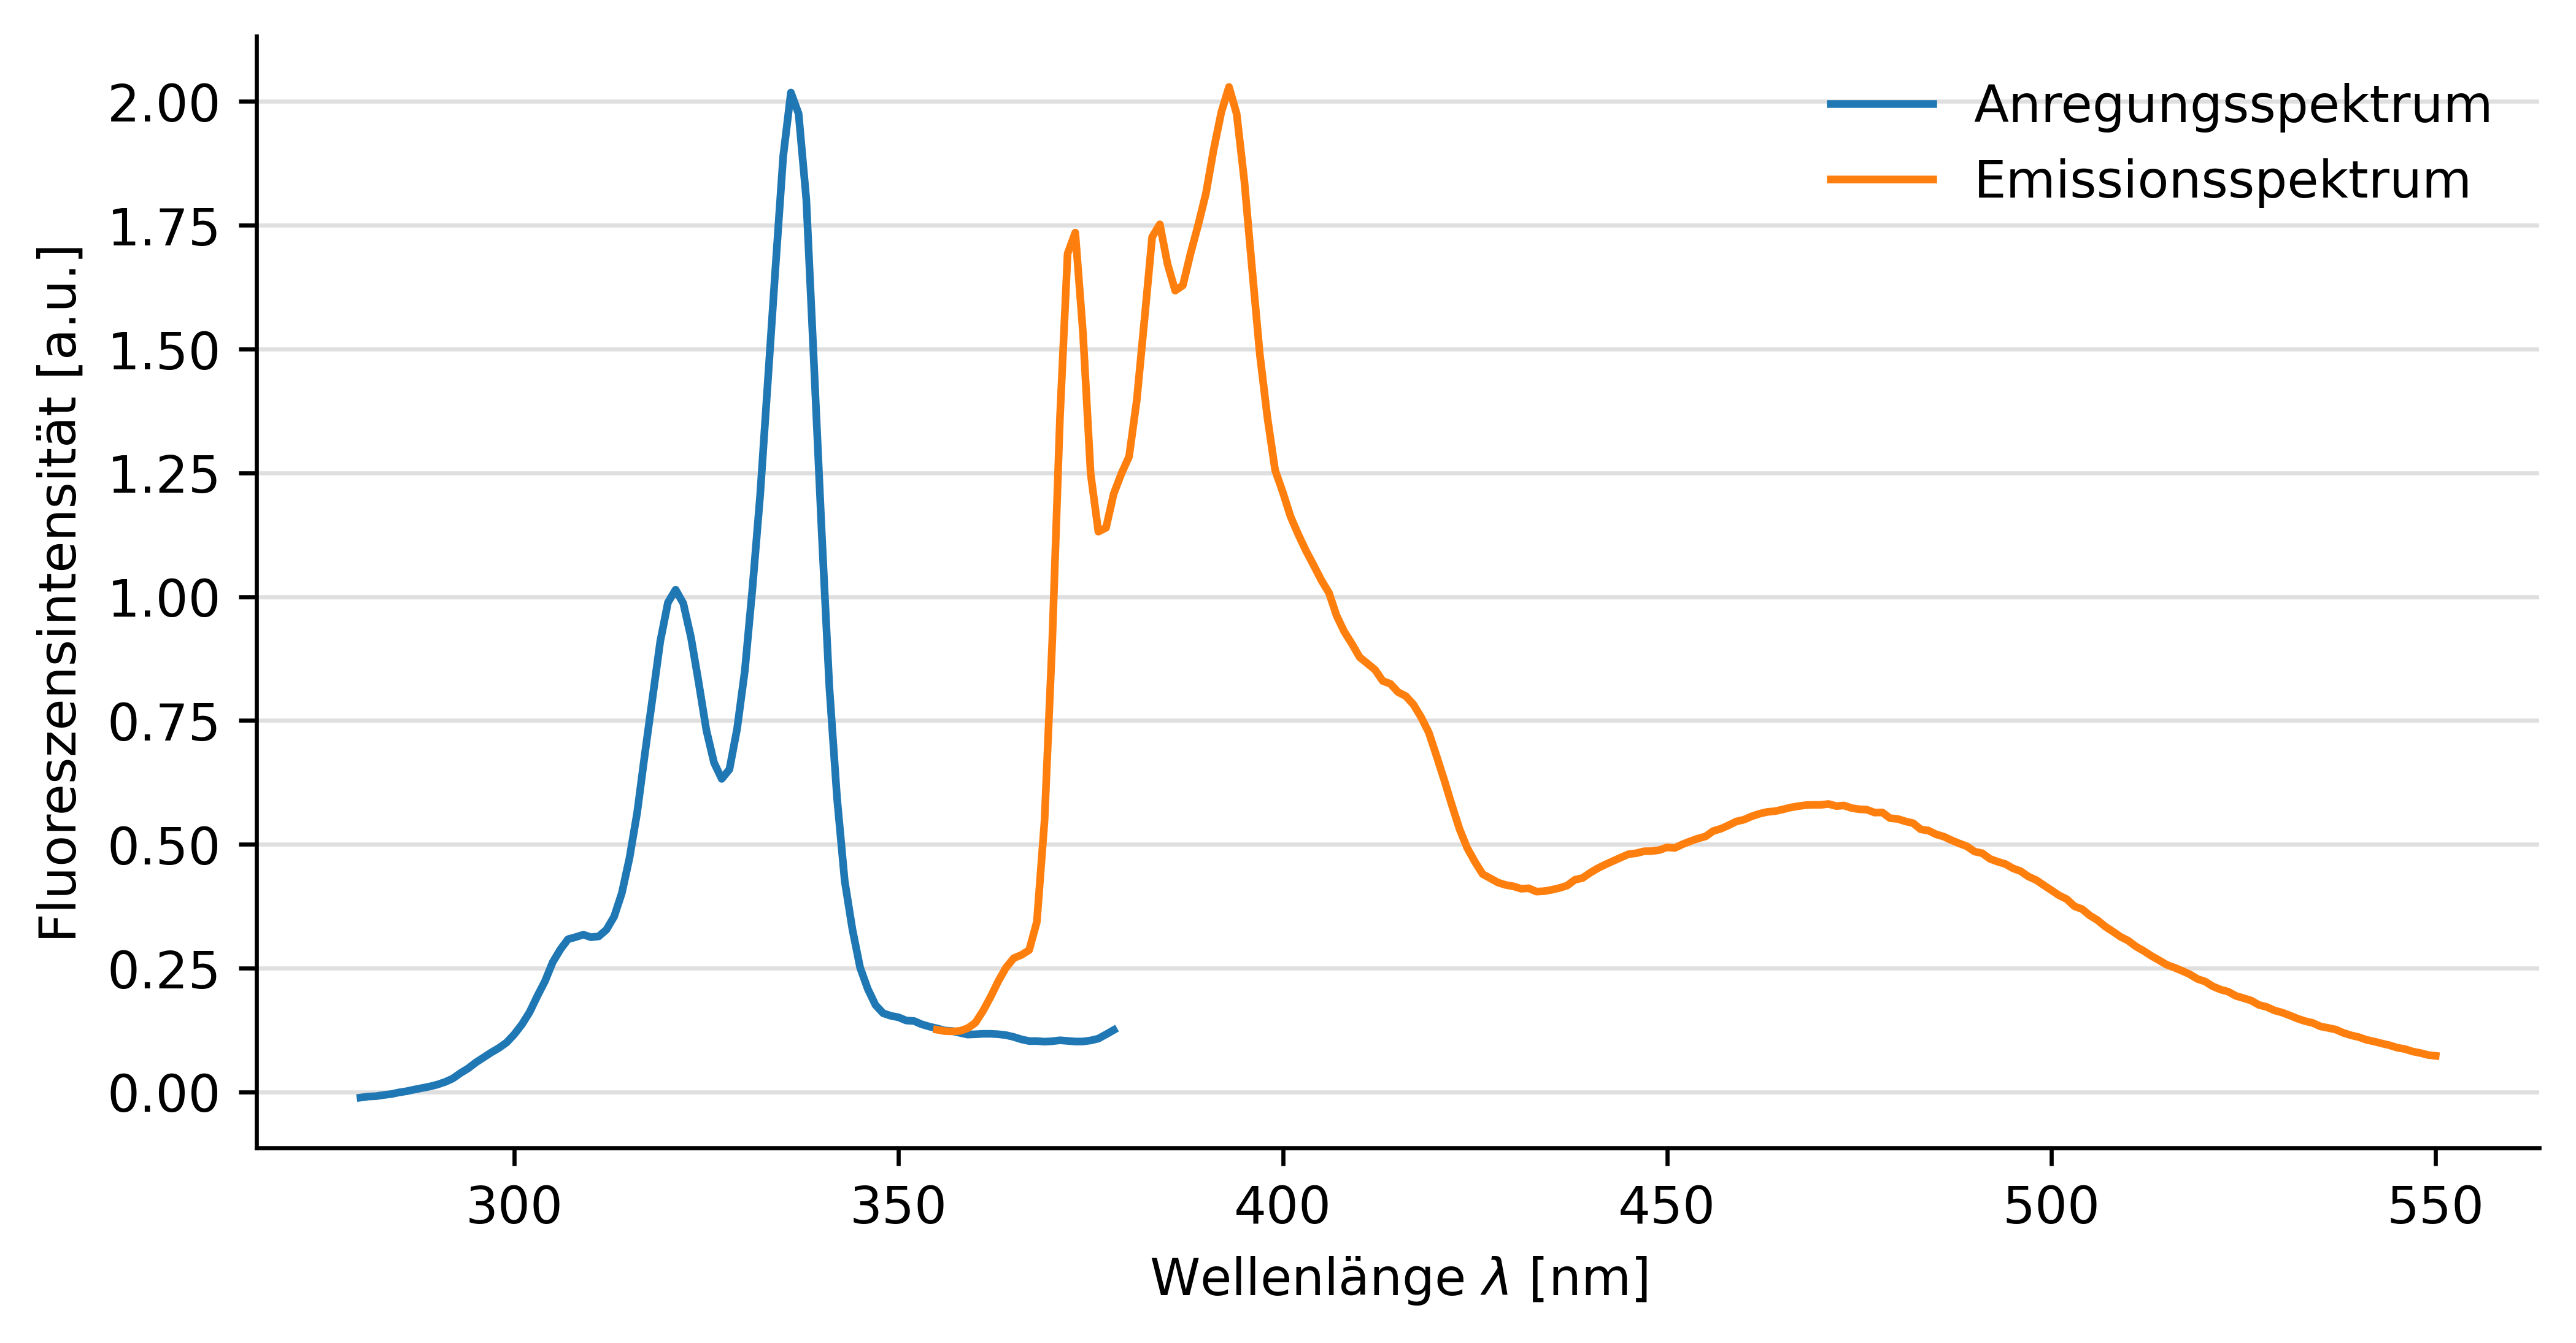
\includegraphics[width=\textwidth]{picture/Em_Ex_Scan_50.png}
			\caption{Anregungs- und Emissionspektrum von Pyren; Verhältnis 1:50 (Pyren:Ei-PC); $T=25^\circ C$, Versorgungsspanung Fluoreszenzspektrometer $U=550V$} 
			\label{Em_Ex_Scan} 
		\end{minipage}
	\end{center}
\end{figure}

\subsection{Fluoreszenzintensitäten des Monomers und des Excimers}
Im Folgenden wurde die Abhängigkeit der Fluoreszenzintensität der Monomere  ($\lambda=393$nm) und Excimere ($\lambda=470$nm) von der Pyrenkonzentration und von der Temperatur untersucht.\\
Am Gerät 3 wurden die Messungen von Pyren in Ei-PC und am Gerät 4 die Messungen von Pyren in DPPC aufgenommen.

\subsubsection{Fluoreszenzintensität als Funktion der Pyrenkonzentration}\label{sec:F_von_C}
In der Abb. \ref{Konz_Scan} sind die pyrenkonzentrationabhängingen Fluoreszenzintensität dargestellt. Die Messpunkte bei $\lambda=393$nm und bei $\lambda=470$nm wurden anschließend in Abb. \ref{Konz_Verh} zusammengetragen.

%ganzheitlicher Fluoreszenzintensität Scan 
\begin{figure}[h!]
	\begin{center}
		\begin{minipage}{0,8\textwidth}
			
			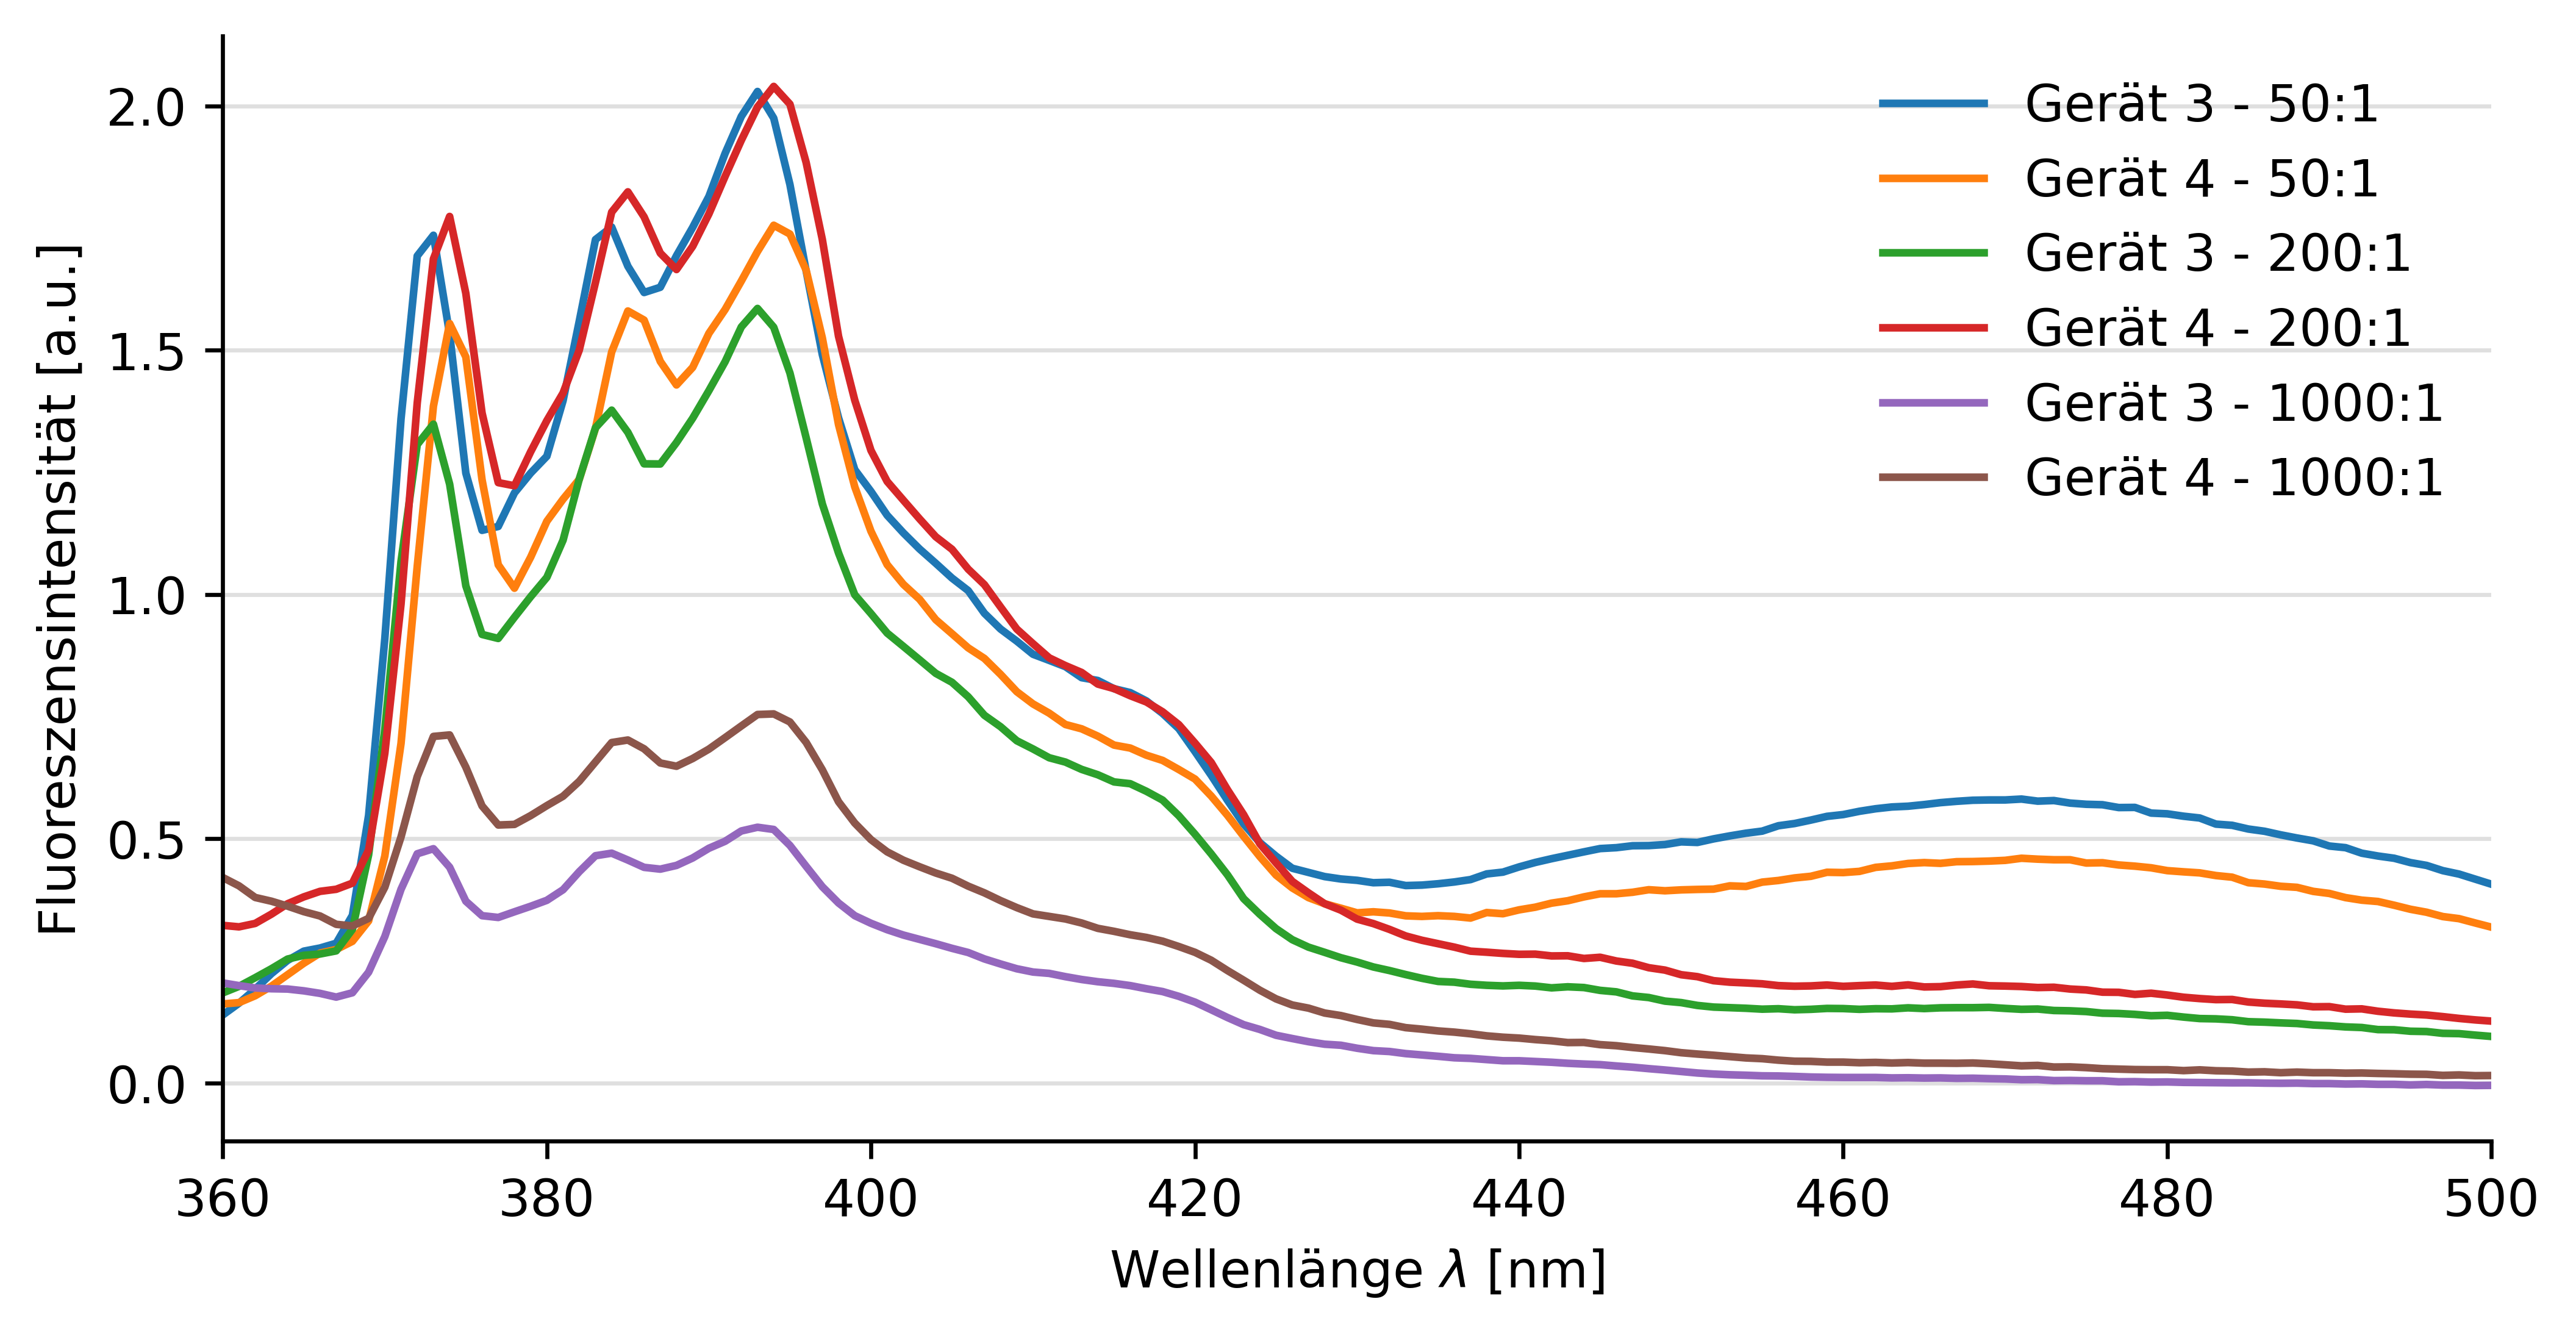
\includegraphics[width=\textwidth]{picture/Konz.png}
			\caption{Fluoreszenzintensität Spektrum von verschiedenen Ei-PC:Pyren-Verhältnissen} 
			\label{Konz_Scan} 
		\end{minipage}
	\end{center}
\end{figure}

%Fluoreszenzintensität als Funktion der Pyrenkonzentration
\begin{figure}[h!]
	\begin{center}
		\begin{minipage}{0,8\textwidth}
			
			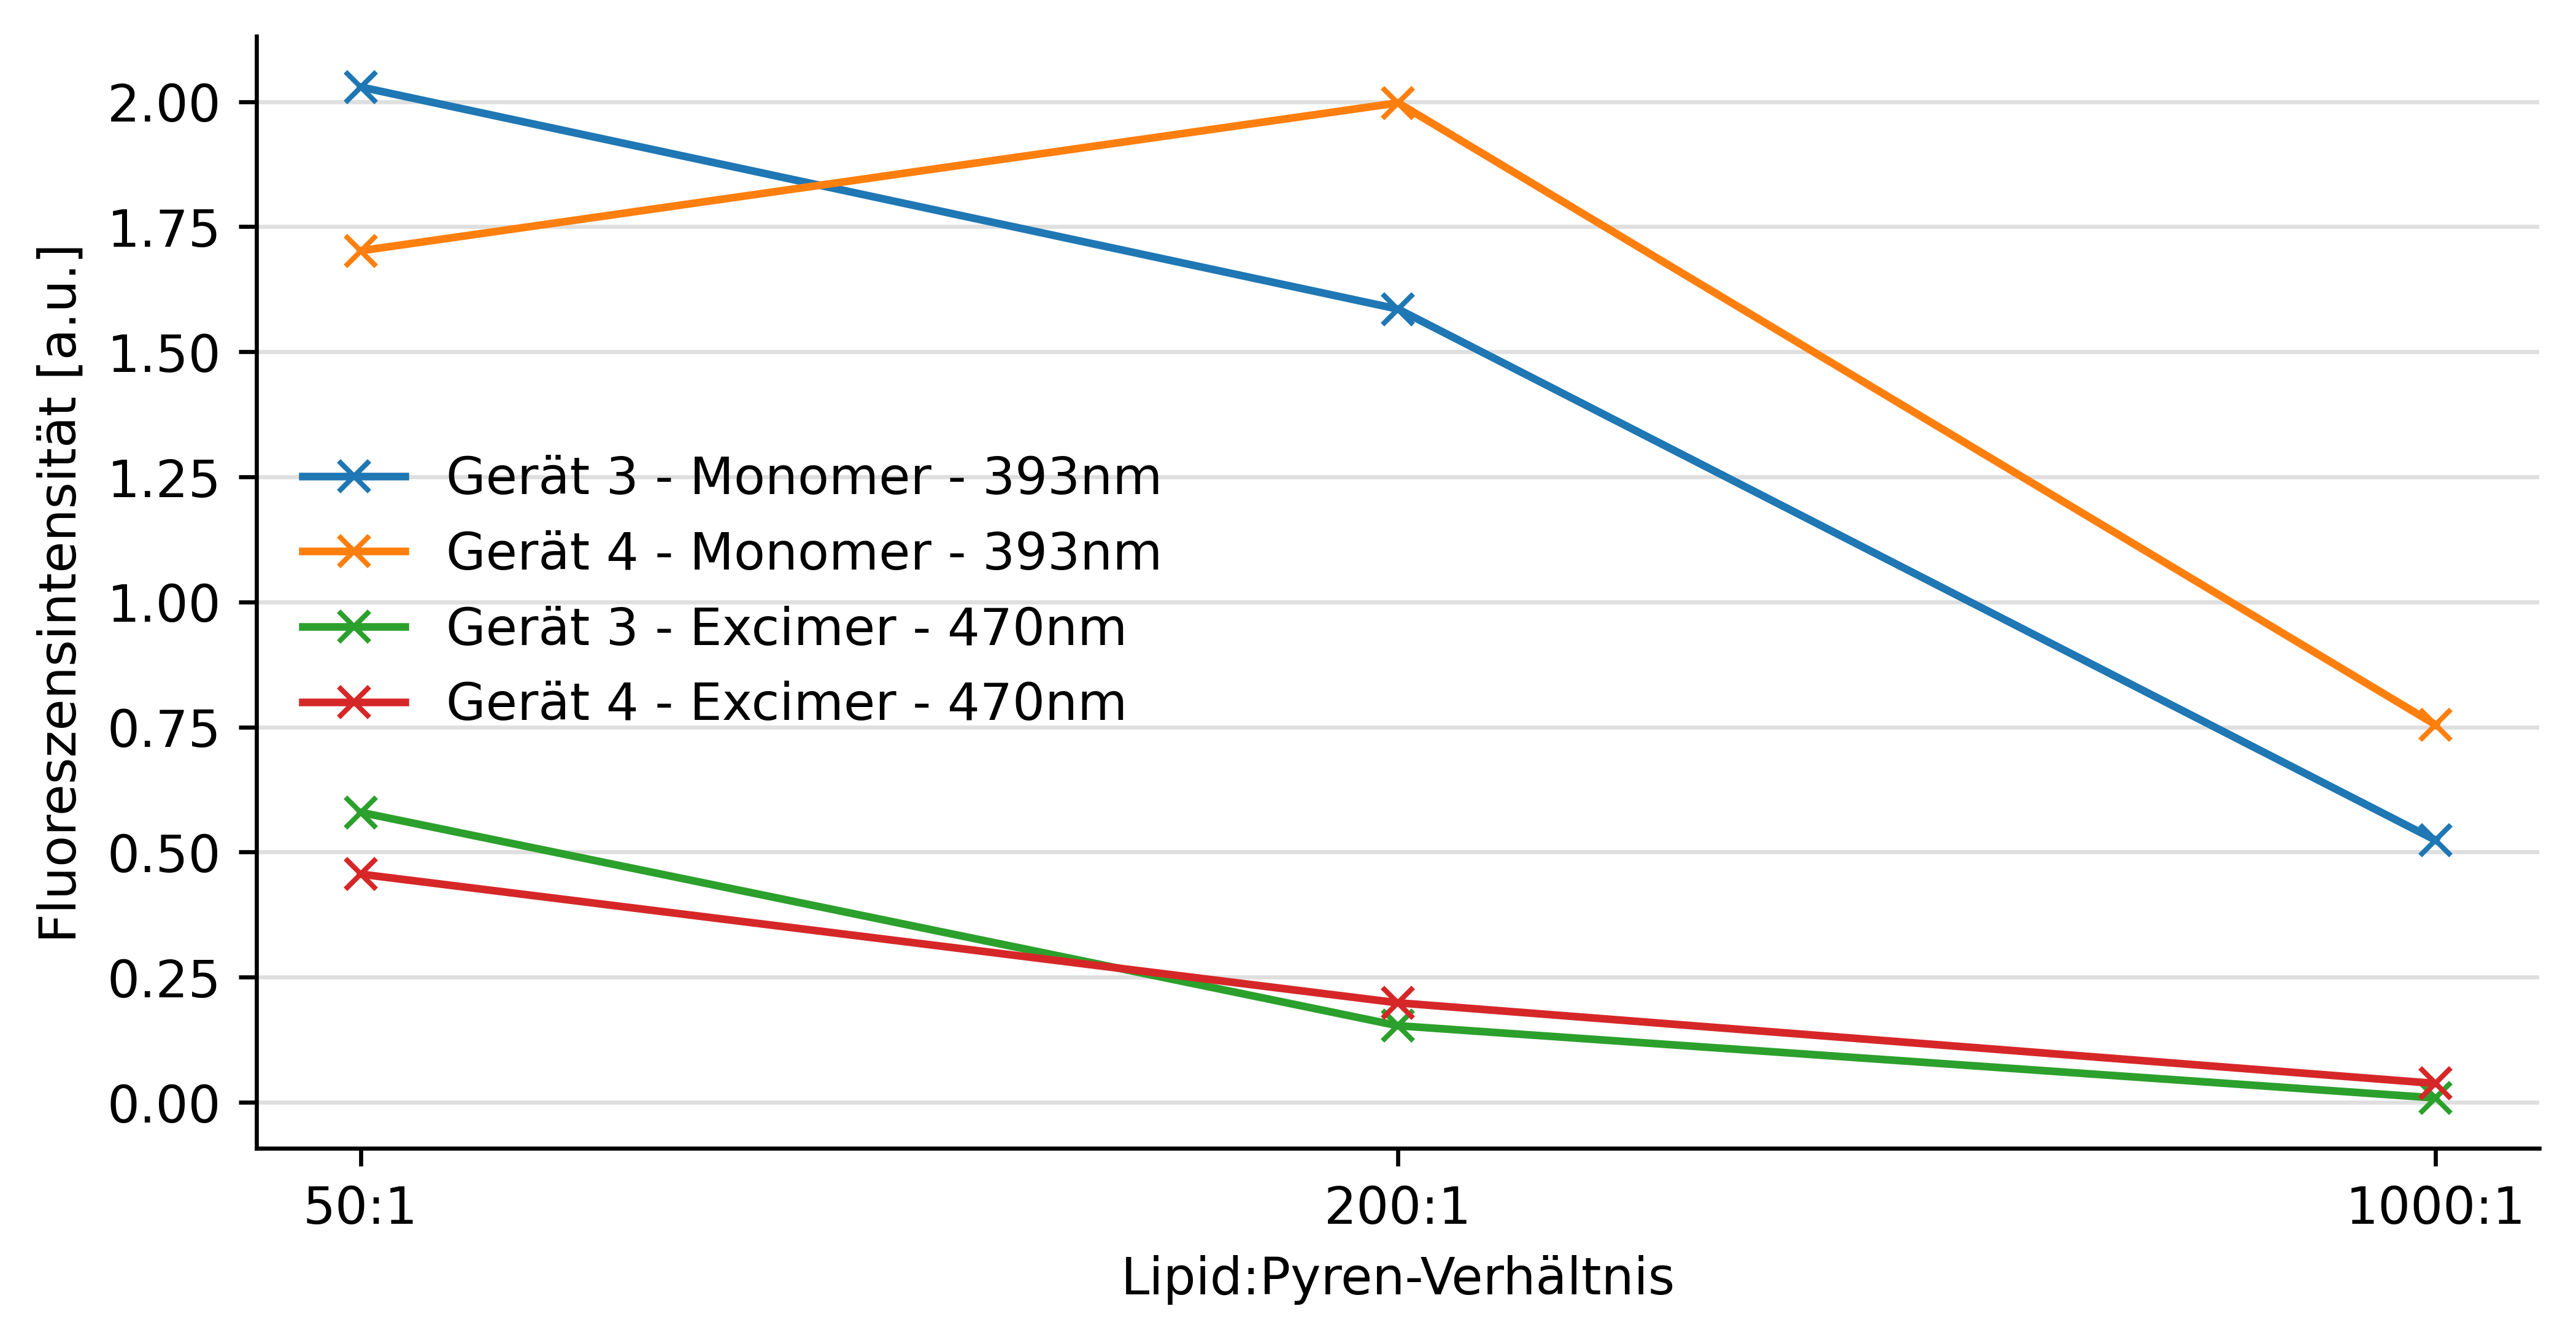
\includegraphics[width=\textwidth]{analysis/reports/Konz_Verh.png}
			\caption{Fluoreszenzintensität als Funktion des Ei-PC:Pyren-Verhältnis} 
			\label{Konz_Verh} 
		\end{minipage}
	\end{center}
\end{figure}
\vspace*{3.4cm}


\subsubsection{Fluoreszenzintensität als Funktion der Temperatur} \label{sec:FvonT}

Analog zum Verfahren aus dem Kapitel \ref{sec:F_von_C} wurden die Fluoreszenzmessdaten (bei Erhöhung der Temperatur im Messsystem) bestimmt und in den Abb. \ref{Monomer_Temp} und Abb. \ref{Excimer_Temp} dargestellt.

%Fluoreszenzintensität des Monomer als Funktion der Temperatur 
\begin{figure}[h!]
	\begin{center}
		\begin{minipage}{0,8\textwidth}
			
			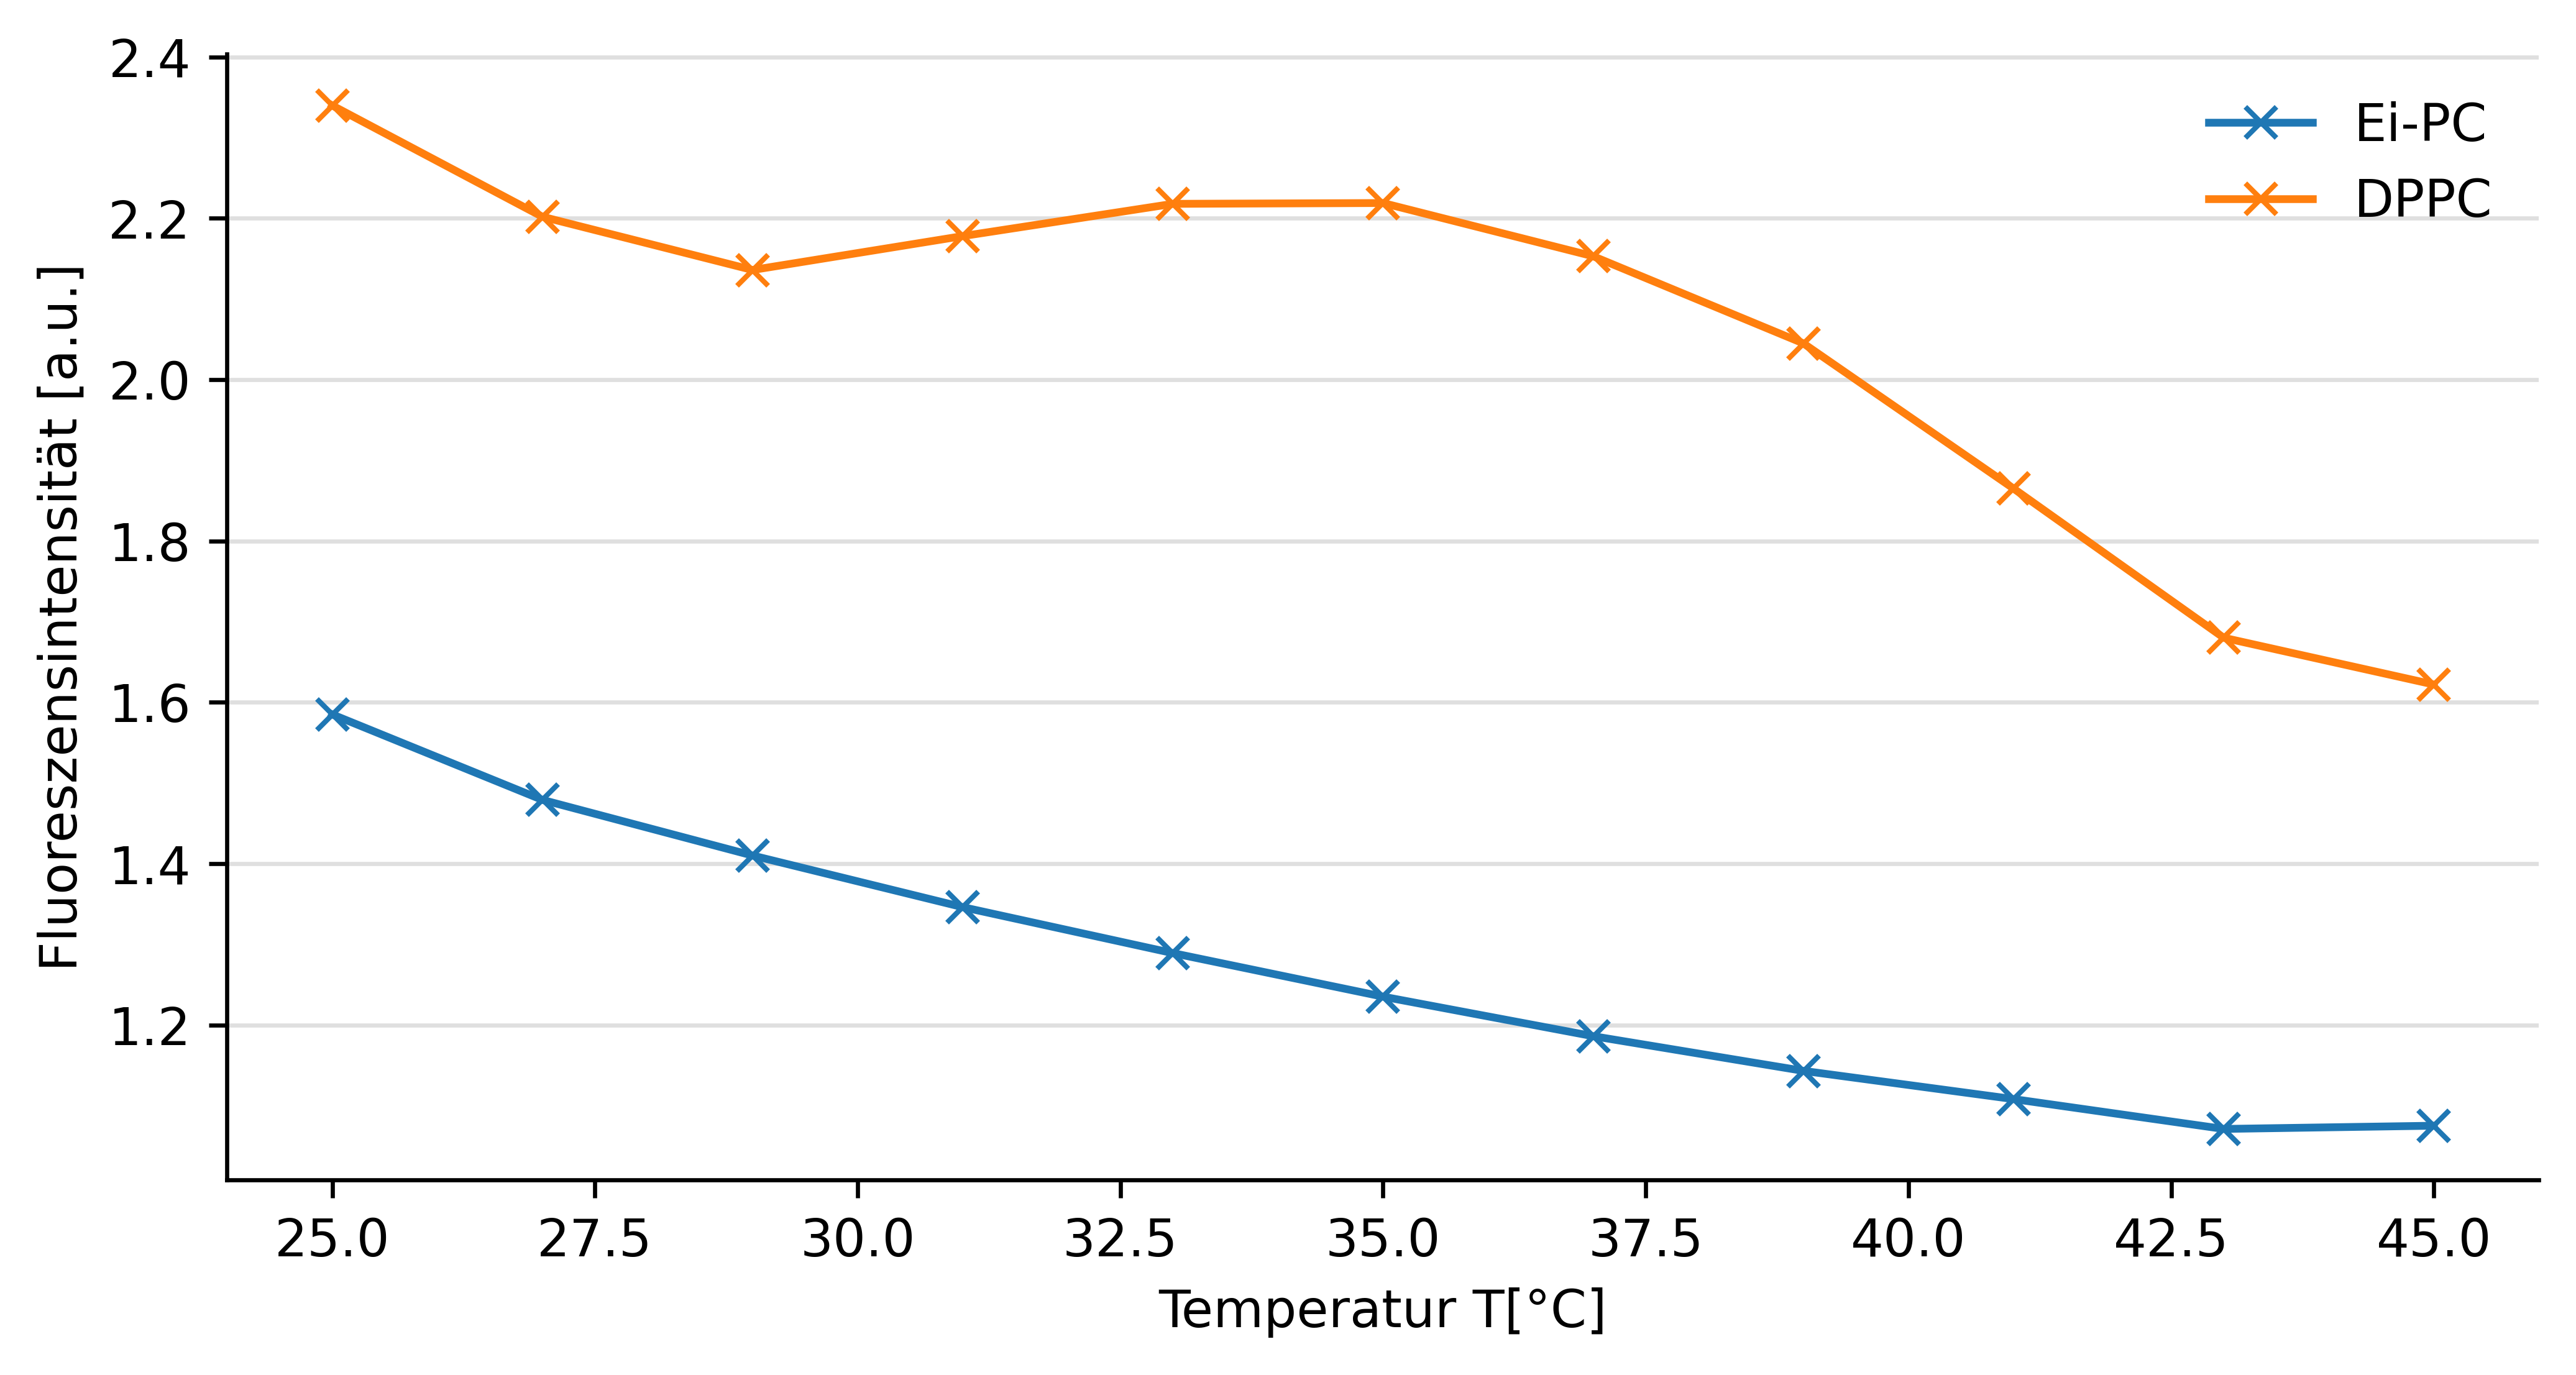
\includegraphics[width=\textwidth]{picture/Monomer_Temp.png}
			\caption{Pyren in Ei-PC bzw. DPPC Vesikeln; Fluoreszenzintensität des Monomer als Funktion der Temperatur} 
			\label{Monomer_Temp} 
		\end{minipage}
	\end{center}
\end{figure}

%Fluoreszenzintensität des Excimer als Funktion der Temperatur 
\begin{figure}[h!]
	\begin{center}
		\begin{minipage}{0,8\textwidth}
			
			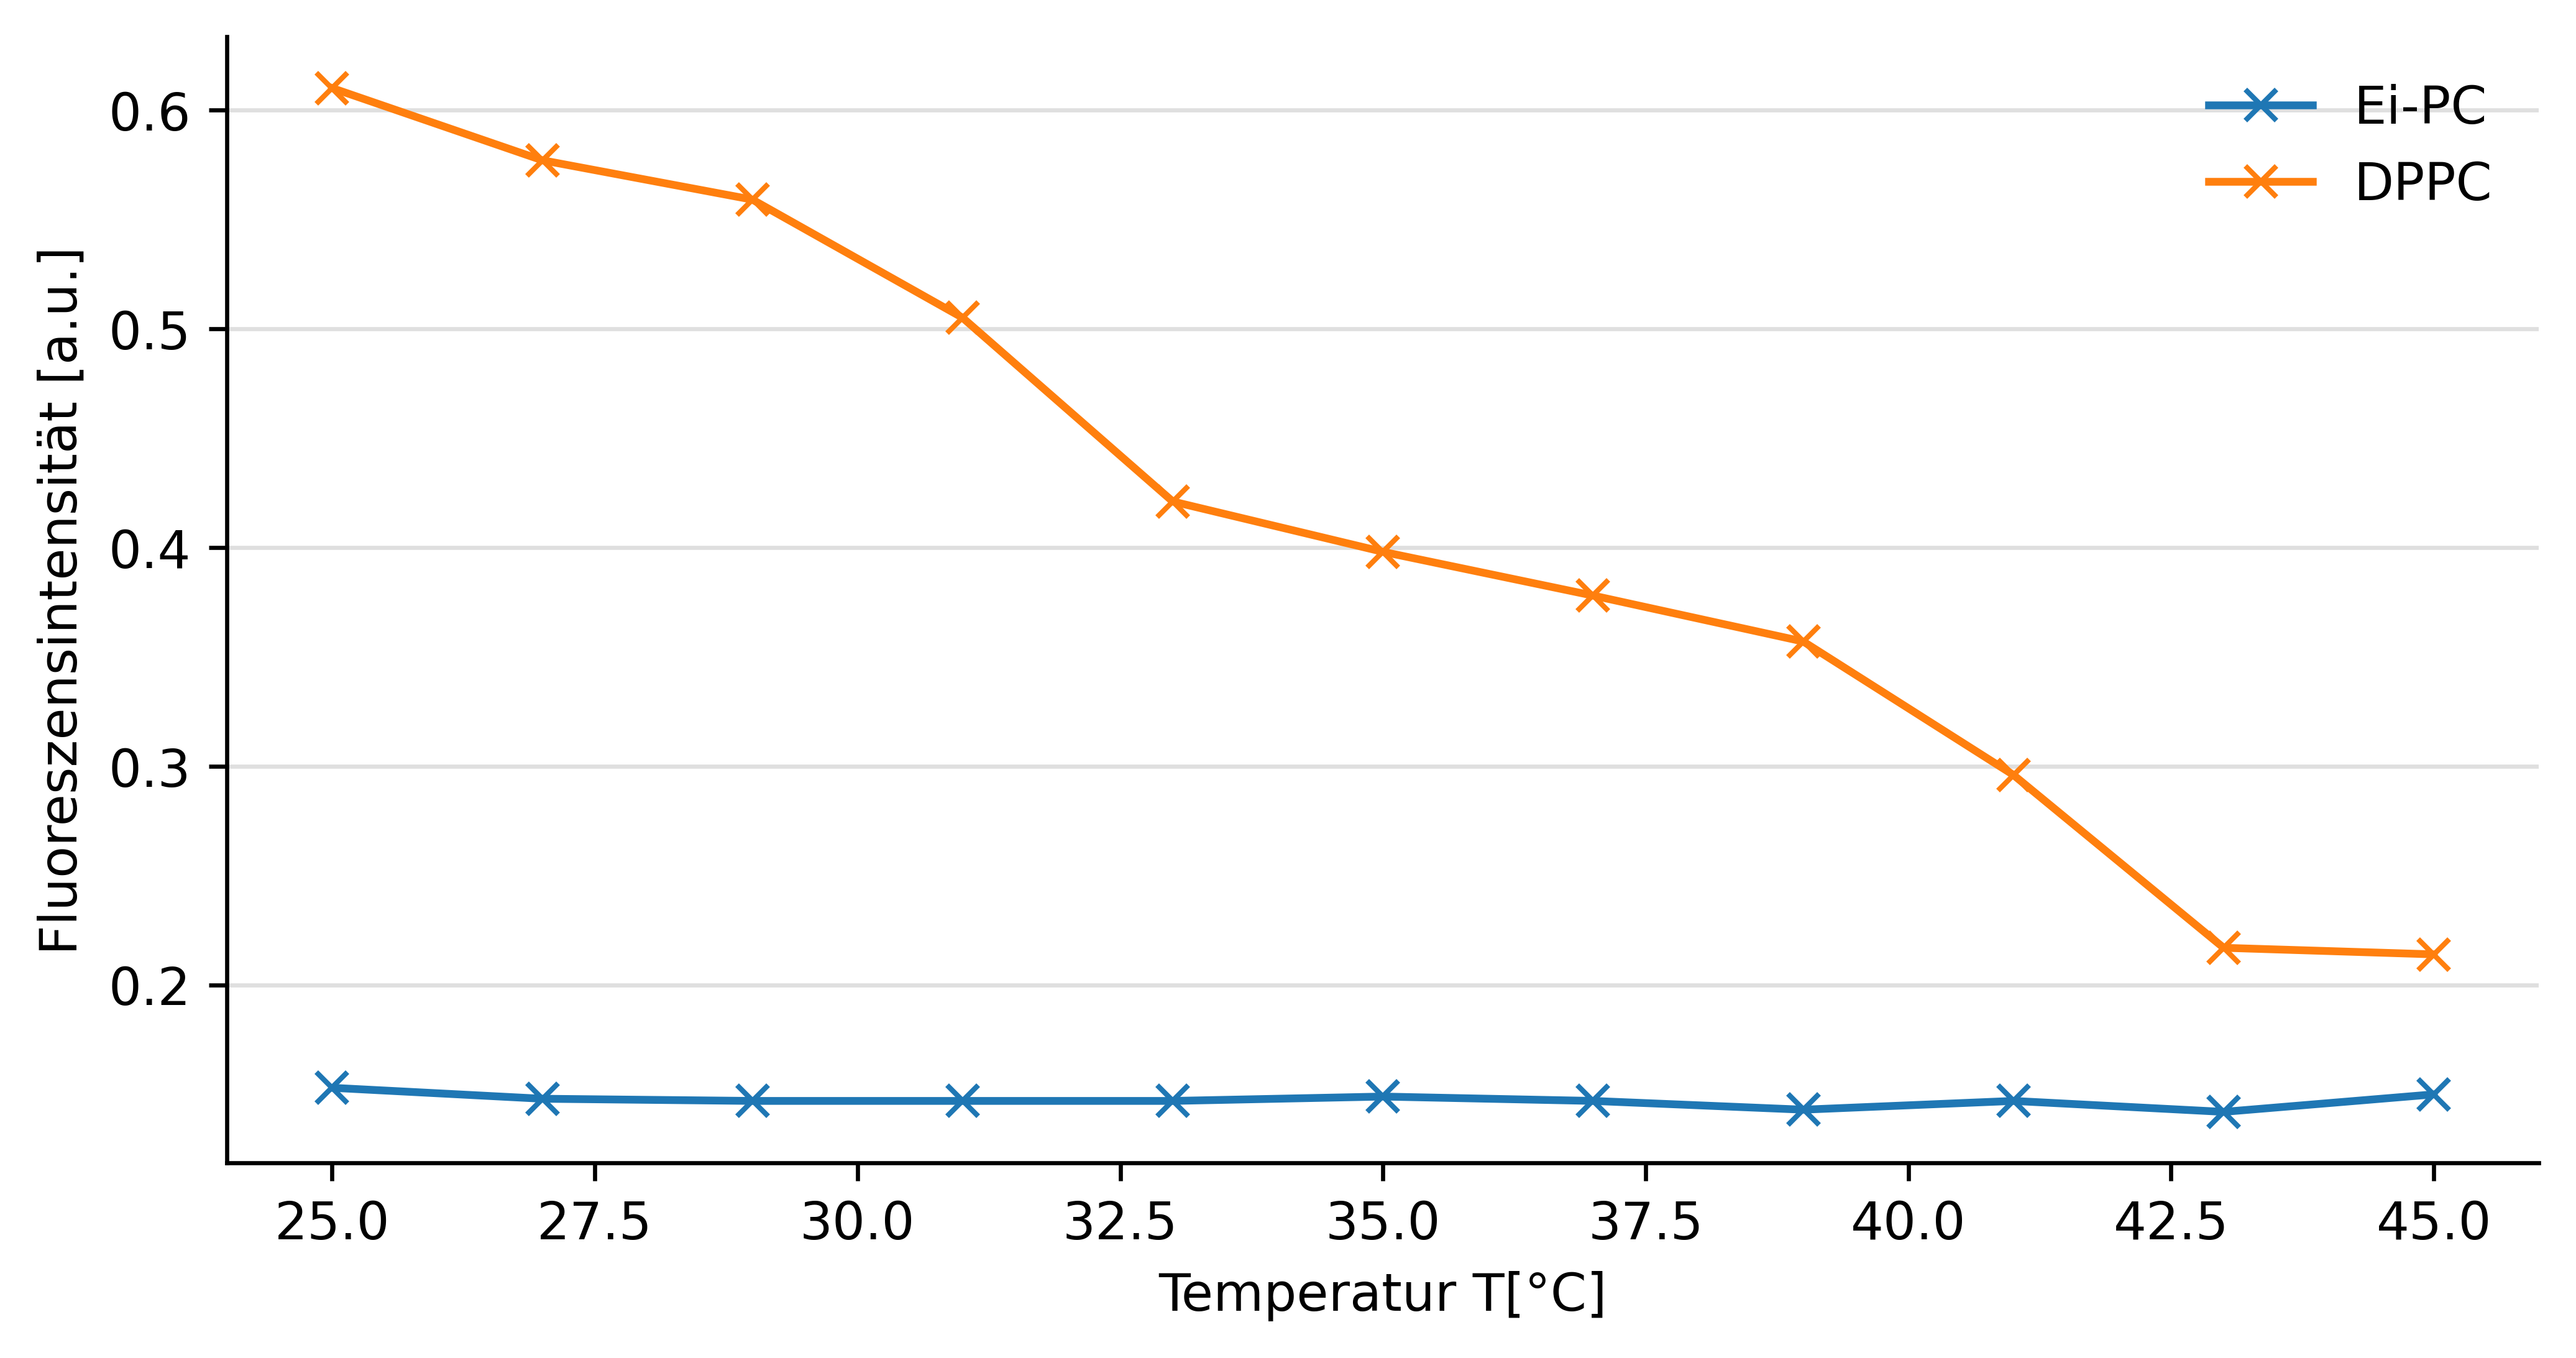
\includegraphics[width=\textwidth]{picture/Excimer_Temp.png}
			\caption{Pyren in Ei-PC bzw. DPPC Vesikeln; Fluoreszenzintensität des Excimer als Funktion der Temperatur} 
			\label{Excimer_Temp} 
		\end{minipage}
	\end{center}
\end{figure}

\subsection{Verhältnis Intensitäten Excimer:Monomer}\label{sec:Ex_Mono}
Folgend aus Kapitel \ref{sec:FvonT} wurde das Verhätlnis von Excimer (Abb. \ref{Excimer_Temp}) zu Monomer (Abb. \ref{Monomer_Temp}) berechnet und in Abb. \ref{Ex_Mono} geplottet.

%Verhältnis Intensitäten Excimer:Monomer für Pyren in Ei-PC bzw. DPPC
\begin{figure}[h!]
	\begin{center}
		\begin{minipage}{0,8\textwidth}
			
			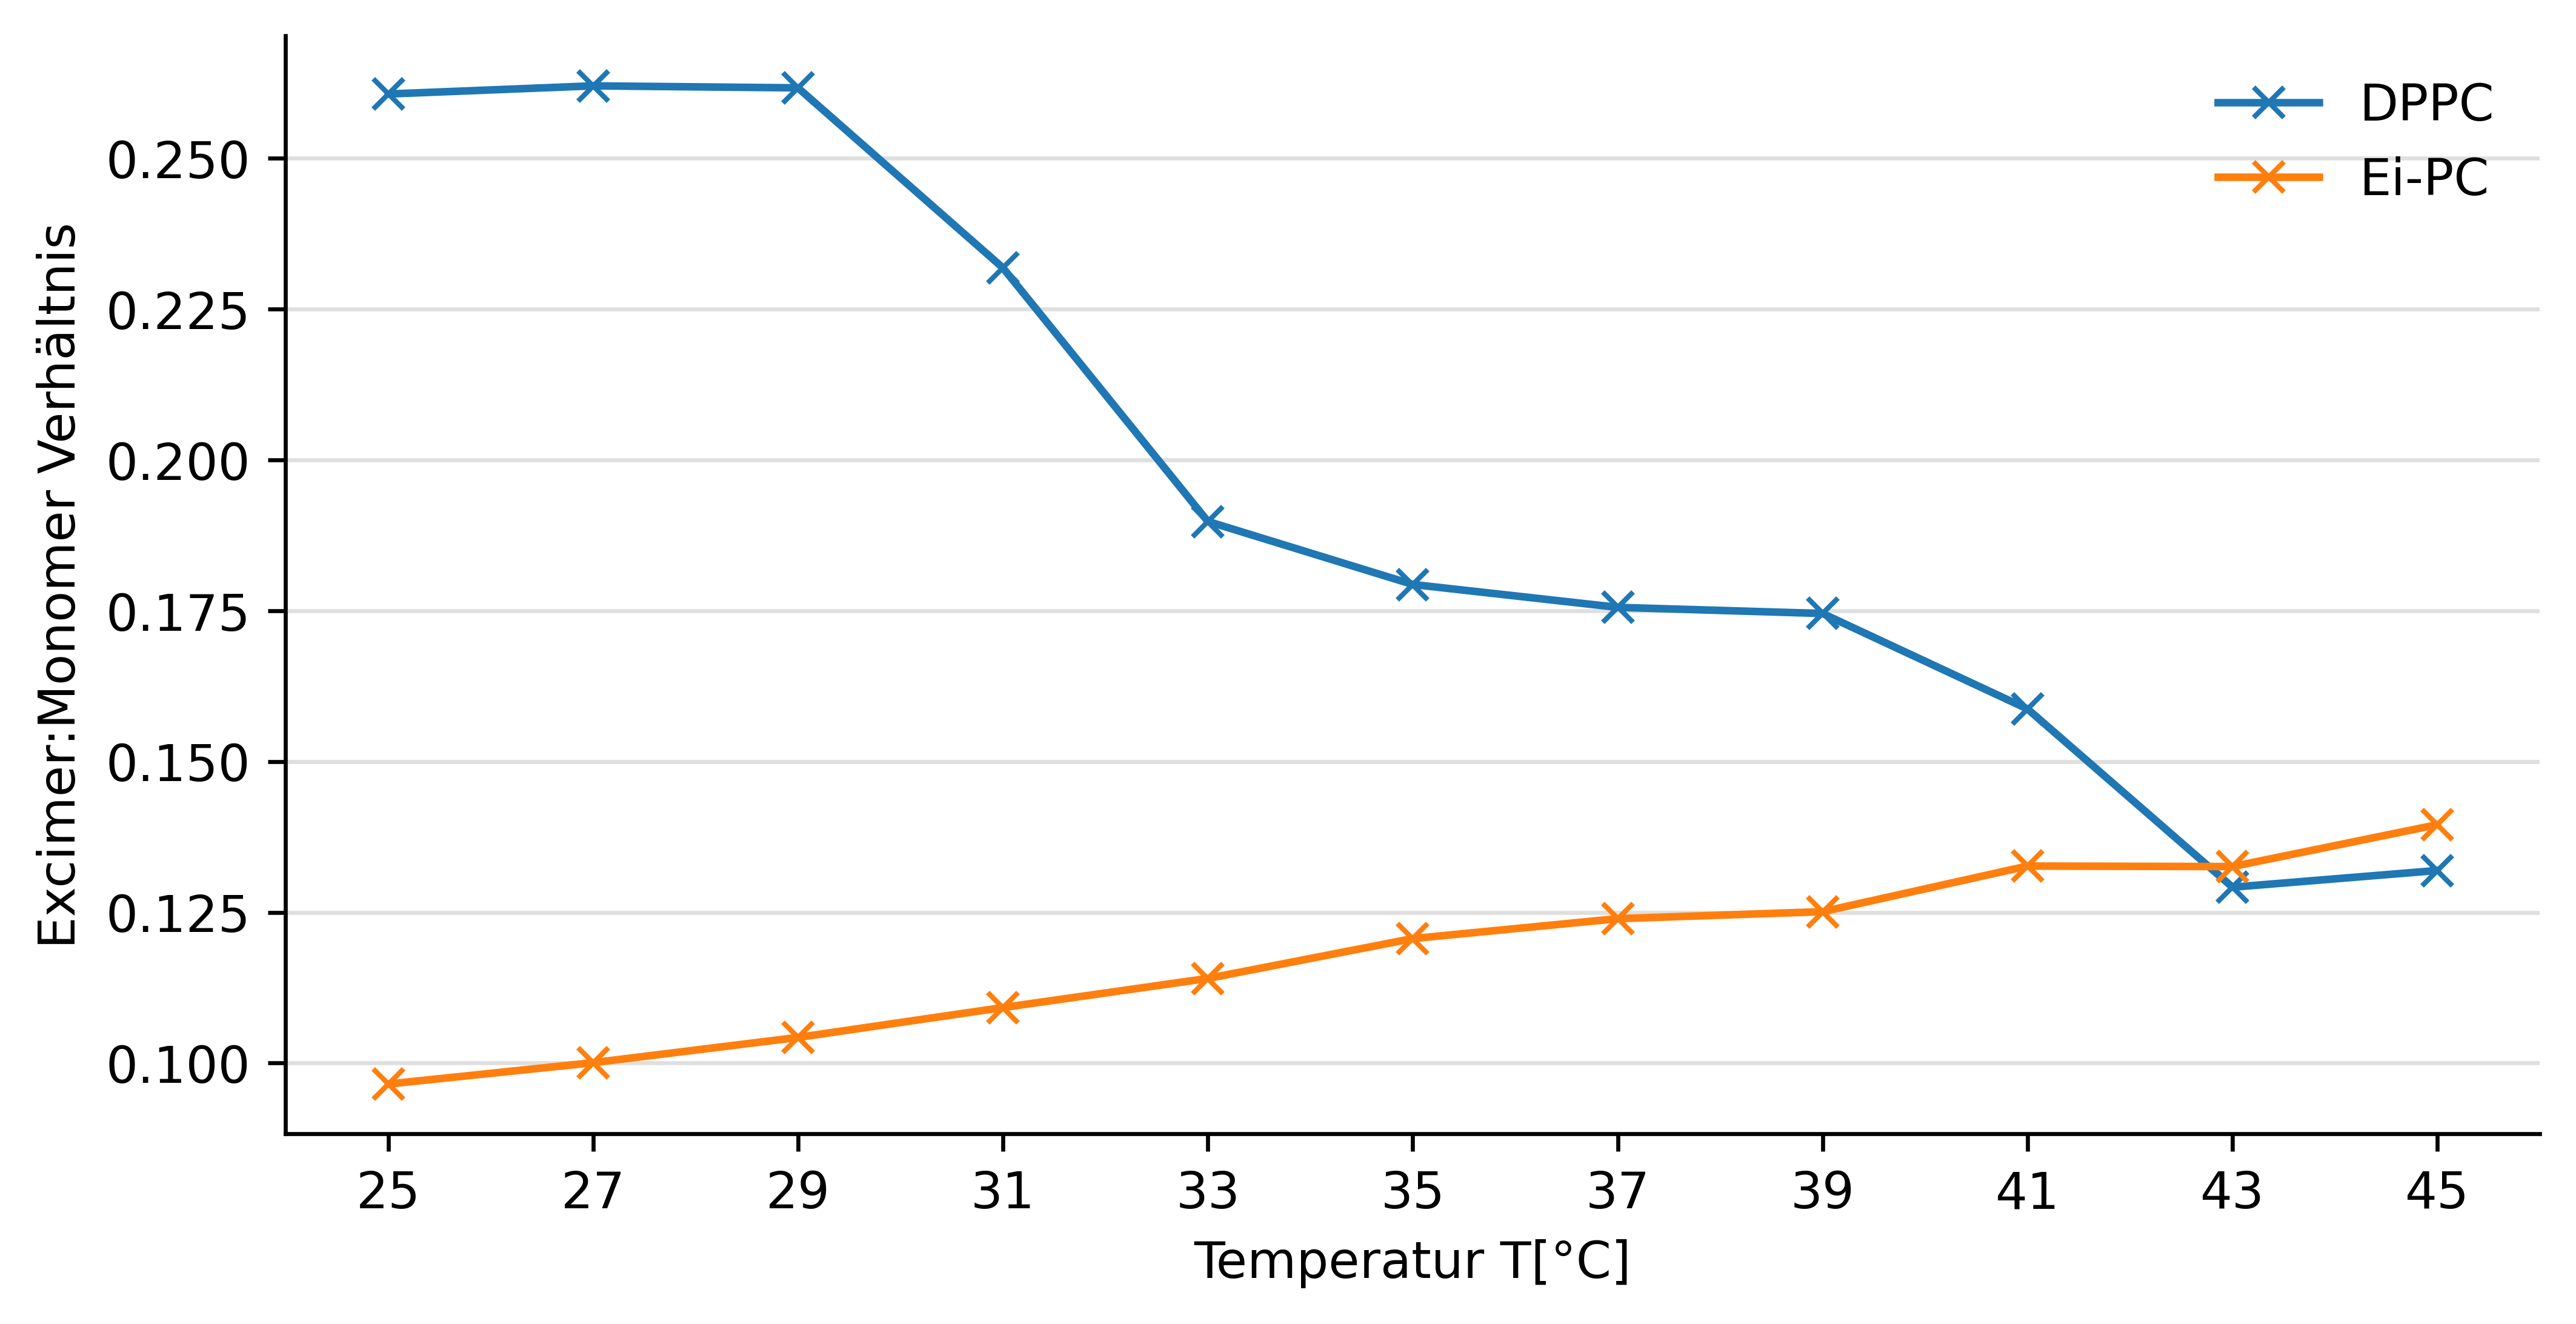
\includegraphics[width=\textwidth]{picture/Ex_Mono.png}
			\caption{Verhältnis Intensitäten Excimer:Monomer für Pyren in Ei-PC bzw. DPPC; Messung der Temperaturabhängigkeit} 
			\label{Ex_Mono} 
		\end{minipage}
	\end{center}
\end{figure}

\subsection{Lateraldiffusionskoeffizienten}
Die Berechnung der temperaturabhängigen Lateraldiffusionskoeffizienten $D_{diff}$ erfolgte analog zum Skript Seite 20 \cite{Kursskript} :\\
Aufbauend auf der Annahme einer $D_{diff}$ als Konzept einer Diffusion auf einem 2D Lipidgitter, wurde die Sprunghaftigkeit $\nu_i$ der Fluorophore von einem Gitterknotenpunkt zum Nächsten über die Formel \ref{formel1}
\begin{equation}\label{formel1}
\nu_i = <n_s> \frac{I'}{I\kappa}\frac{1}{\tau_0}\frac{k_f}{k_{f'}}
\end{equation}
mit der Formel \ref{formel2} 
\begin{equation}\label{formel2}
<n_s>=\frac{2}{\pi X_{py}}ln\frac{2}{X_{py}}
\end{equation}
zur Berücksichtigung der mittleren Sprungszahl zwischen zwei Kollisionen $<n_s>$  hinzugezogen.\\
$D_{diff}$ wurde anschließend über Formel \ref{formel3} berechnet.
\begin{equation}\label{formel3}
D_{diff}=\frac{1}{4}\nu_i \lambda^2
\end{equation}
Es gilt, dass die durchschnittliche Distanz im Lipidgitter $\lambda=0.8\text{nm}$, die Proportionalitätskonstante $\kappa=0.5$ und das Verhältnis der Fluoreszenzübergangsrate des Monomers bzw. Excimers $\frac{k_f}{k_{f'}}=0.1$ beträgt.\\\\
Formel \ref{formel1} und \ref{formel2} wurden anschließend mit den Parametern in die Formel \ref{formel3} eingesetzt und entsprechend gekürzt. \\
 Die temperaturabhängigen Fluoreszenzlebenszeiten des Excimers $\tau_0$
  \begin{table} [h]
 	\footnotesize
 	\begin{center}
 		\caption{Fluoreszenzlebenszeiten $\tau_0$ des Pyren-Excimers; temperaturabhängig}
 		\begin{tabular} {c c c l l l l l}
 			T[$^\circ$C]&  $\tau_0$ [ns] \\ \hline
 			25& 130 \\ \hline 
 			35&	115 \\ \hline 
 			45&	100 \\ \hline 
 		\end{tabular}
 		\label{tab:Lebenszeiten}
 	\end{center}
 \end{table}
wurden dem Skript entnommen.\\
Die Berechnung von $D_{diff}$ abhängig des molaren Anteils von Pyren $X_{py}$ und des in \ref{sec:Ex_Mono} berechneten Excimer:Monomer Verhältnissen (welche $\frac{I'}{I}$ entsprechen) erfolgte durch die gewonnene Formel \ref{formel4}

\begin{equation}\label{formel4}
D_{diff}=0.1\frac{1}{\pi X_{py}}ln\left(\frac{2}{X_{py}}\right)\frac{I'}{I}\frac{1}{\tau_0}\cdot0.64\text{nm}^2
\end{equation}
$X_{py}$ für die Messdaten zu Ei-PC und DPPC betrugen $X_{py}=5\cdot 10^{-3}$ 
%und für DPPC, da es bei annähernd gleicher Molaren Masse aber in 10-facher Menge vorhanden war, \\
%$X_{py,DPPC}=5\cdot 10^{-4}$. \\
Die jeweiligen Ergebnisse sind in der Tabelle \ref{tab:meinetabelle} dargestellt.

 \begin{table} [h]
	\footnotesize
	\begin{center}
		\caption{errechnete Diffusionskoeffizienten $D_{diff}$ von Pyren für ausgewählte Temperaturen}
		\begin{tabular} {c c c l l l l l}
			T[$^\circ$C]&  \multicolumn{2}{c}{$D_{diff}$ [$m^2s^{-1}$]} & \\ \hline
			&	Ei-PC&	DPPC \\ \hline 
			25&	1,81E-11&	1,15E-10\\ \hline 
			35&	2,56E-11&	8,45E-11\\ \hline 
			45&	3,41E-11&	5,23E-11\\ \hline 
		\end{tabular}
		\label{tab:meinetabelle}
	\end{center}
\end{table}


\newpage

	\section{Diskussion}
%Diskussion: Einordnung der Ergebnisse und beobachteten Effekte sowohl zueinander als auch in Bezug auf die allgemeine Literatur. Beantwortung %der Fragen dem Skript. Fehlerbetrachtung/-abschätzung.
In Abb. \ref{Ex_Mono} bei DPPC sieht man 2 Übergänge. Einen bei $T=35^\circ C$ und einen bei  $T=43^\circ C$. Der Erste kann ein Artefakt sein bzw. vielleicht kann man darin auch die Ripple Phase $P_{\beta '}$ sehen. Eine engmaschigere Messreihe würde für Klarheit sorgen.\\
Ein Vergleich der temperaturabhängigen Fluoreszenzintensitäten von Pyren in DPPC (Abb. \ref{Temp_Geraet4}) mit Pyren in Ei-PC (Abb. \ref{Temp})
zeigt auf, dass sich bei DPPC die Fluoreszenzintensität des Excimerpeaks bei $\lambda=470$nm mit zunehmender Temperatur abnimmt, während bei Ei-PC die Fluoreszenzintensität des Excimerpeaks konstant bleibt. \\
Ei-PC  besitzt gegenüber DPPC(16:0) über ungesättigte Fettsäuren mit cis-Bindungen, die eine Störung der Anordnung der Lipide in der Membran darstellen. Ei-PC verbleibt deswegen bei den Experimentbedingungen im flüssig-kristallinen Zustand $L_\alpha$. 
DPPC befindet sich bei $T=25^\circ C$ in der $L_{\beta '}$ Phase und wandelt sich ab circa $T=43^\circ C$ in $L_\alpha$ um, was man indirekt aus der Abb. \ref{Ex_Mono} herauslesen kann. \\
 DPPC(16:0) besteht aus gesättigten Acylketten, worin Pyren wohl nicht richtig Platz findet. Dies deutet auf ein Clustering von Pyren bei DPPC in $L_{\beta '}$ hin, wodurch sich die bei geringeren Temperaturen höheren Fluoreszenzintensitäten im Vergleich zu dem Ei-PC / Pyren System erklären. \\
Für eine eindeutige Aussage bezüglich der Phasenumwandlung ist die Technik  des vorliegenden Experiment als alleinstehende Methode weniger geeignet. Die möglichen Phasenumwandlungspunkte für DPPC von $L_{\beta '} \rightarrow P_{\beta '}$ und von $P_{\beta '} \rightarrow L_\alpha$ stimmen aber annäherend mit den Literaturwerten von $36^\circ C$ ($L_{\beta '} \rightarrow P_{\beta '}$) und $41.3^\circ C$ ($P_{\beta '} \rightarrow L_\alpha$) überein \cite{Biltonen1993}.\\


%Temperaturplot Pyren in DPPC
\begin{figure}[h!]
	\begin{center}
		\begin{minipage}{0,8\textwidth}
			
			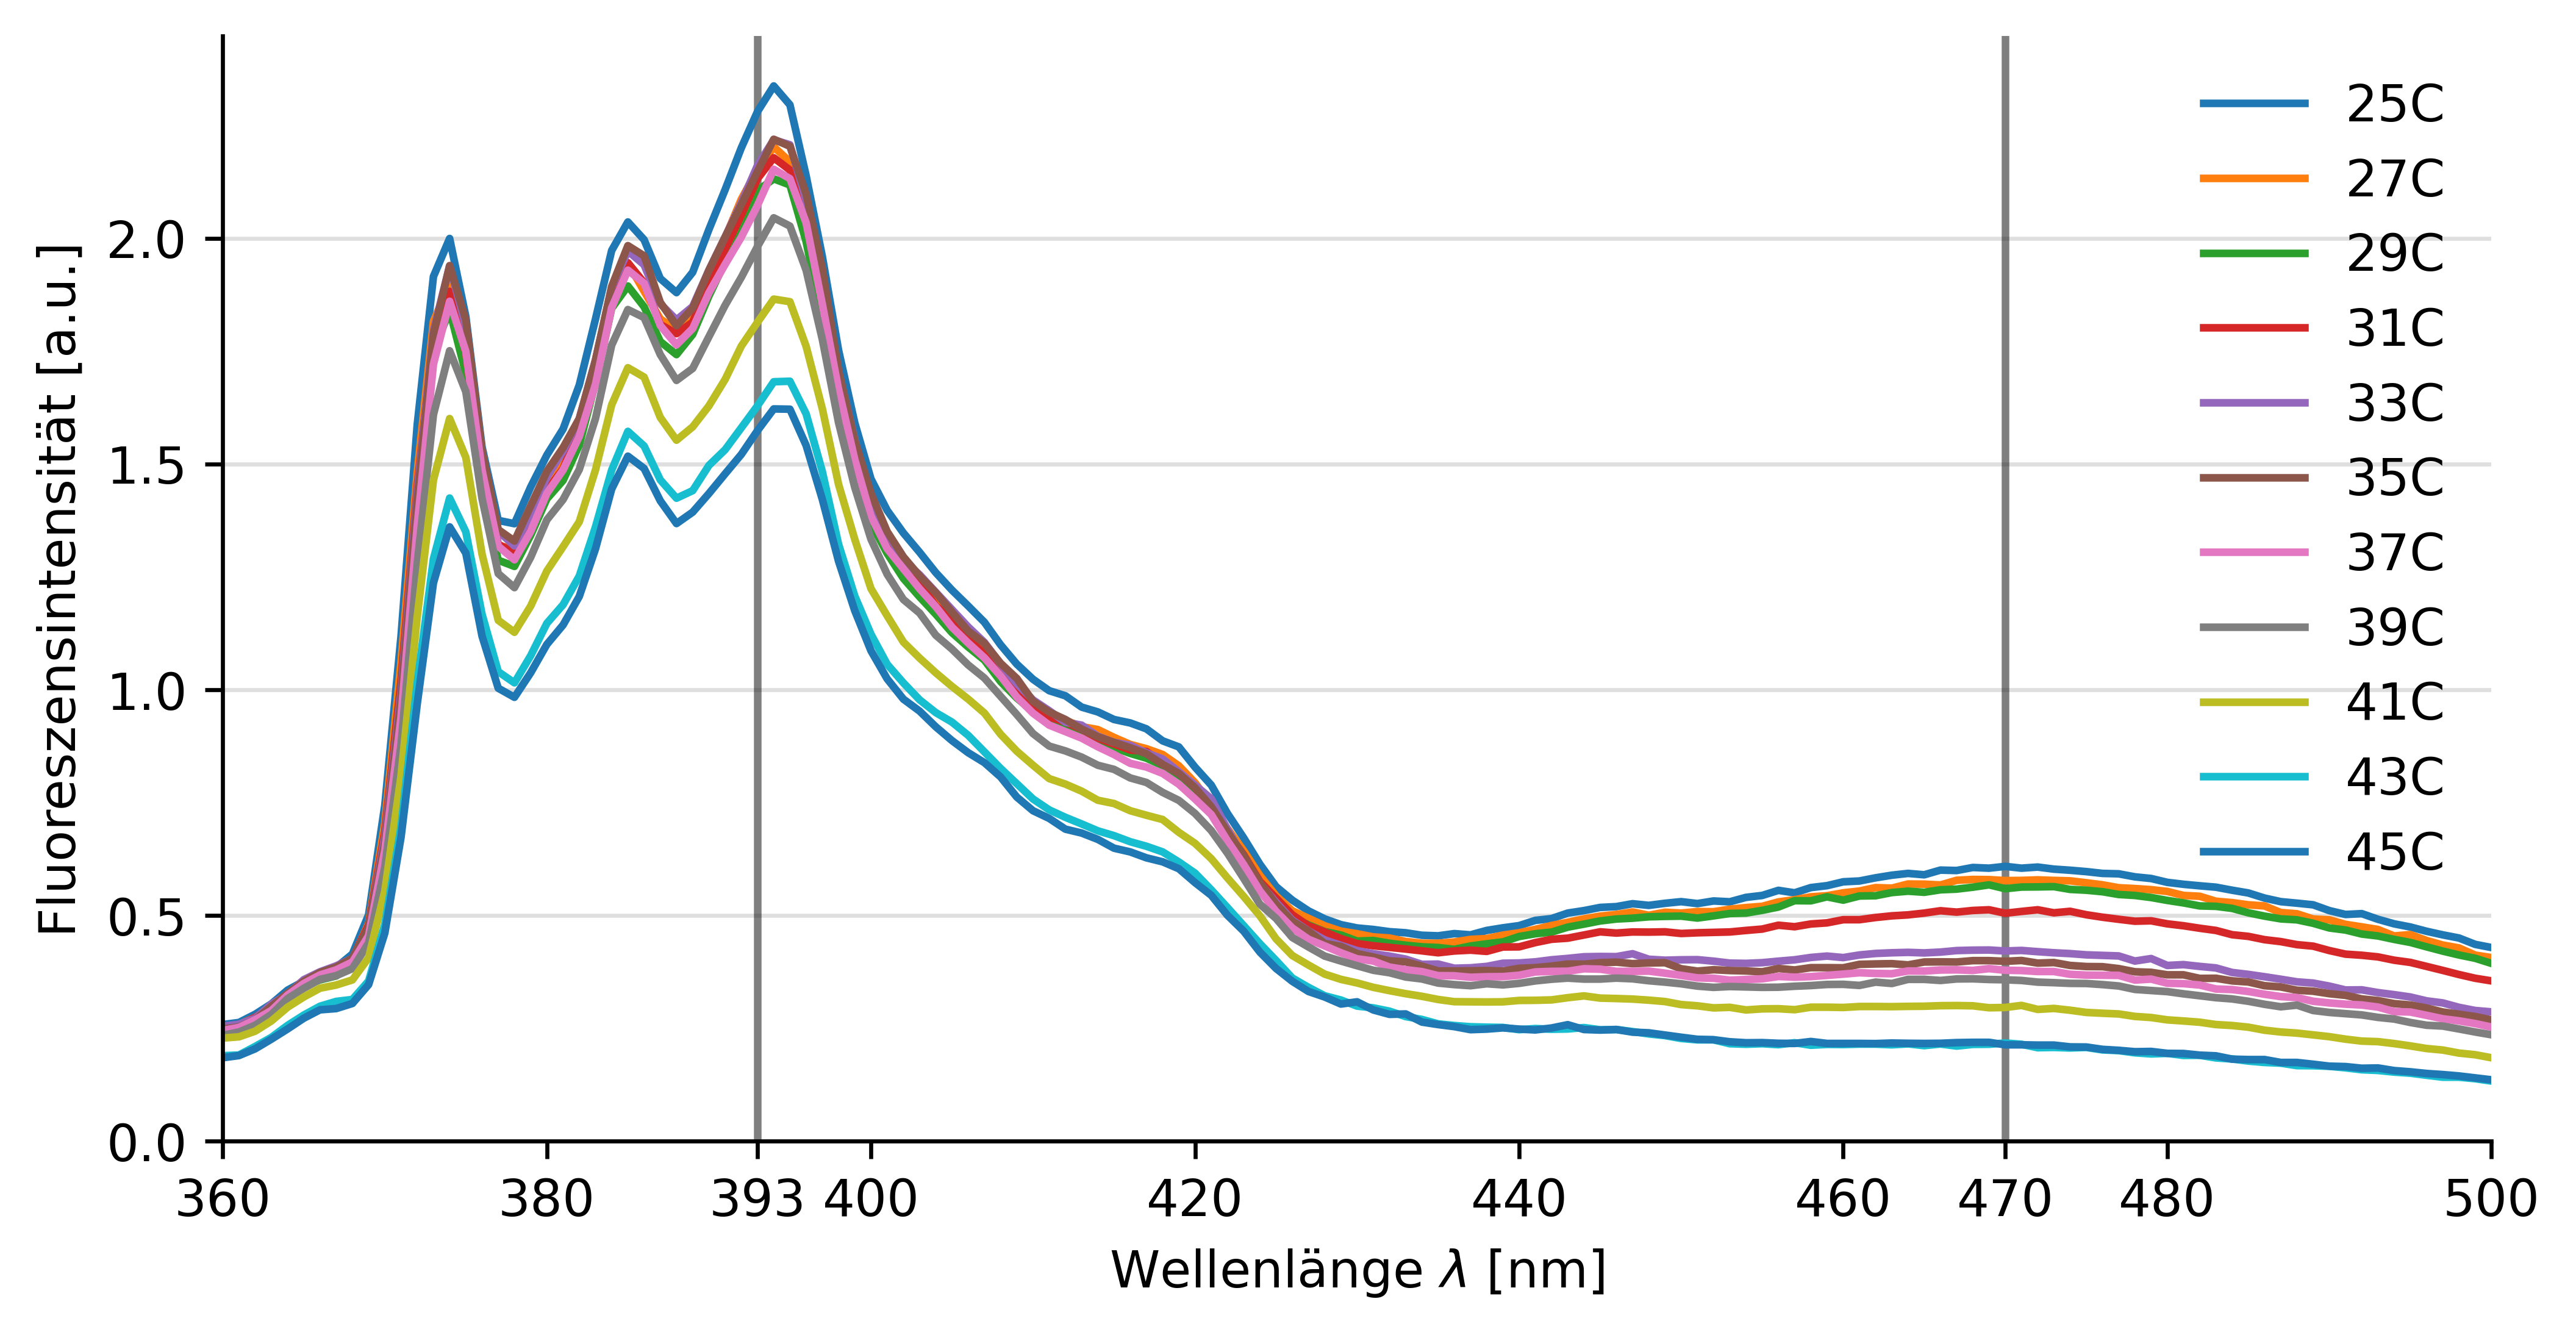
\includegraphics[width=\textwidth]{picture/Temp_Geraet4.png}
			\caption{Fluoreszenzintensität Spektrum von Pyren in DPPC; temperaturabhängig} 
			\label{Temp_Geraet4} 
		\end{minipage}
	\end{center}
\end{figure}
\begin{figure}[h!]
	\begin{center}
		\begin{minipage}{0,8\textwidth}
			
			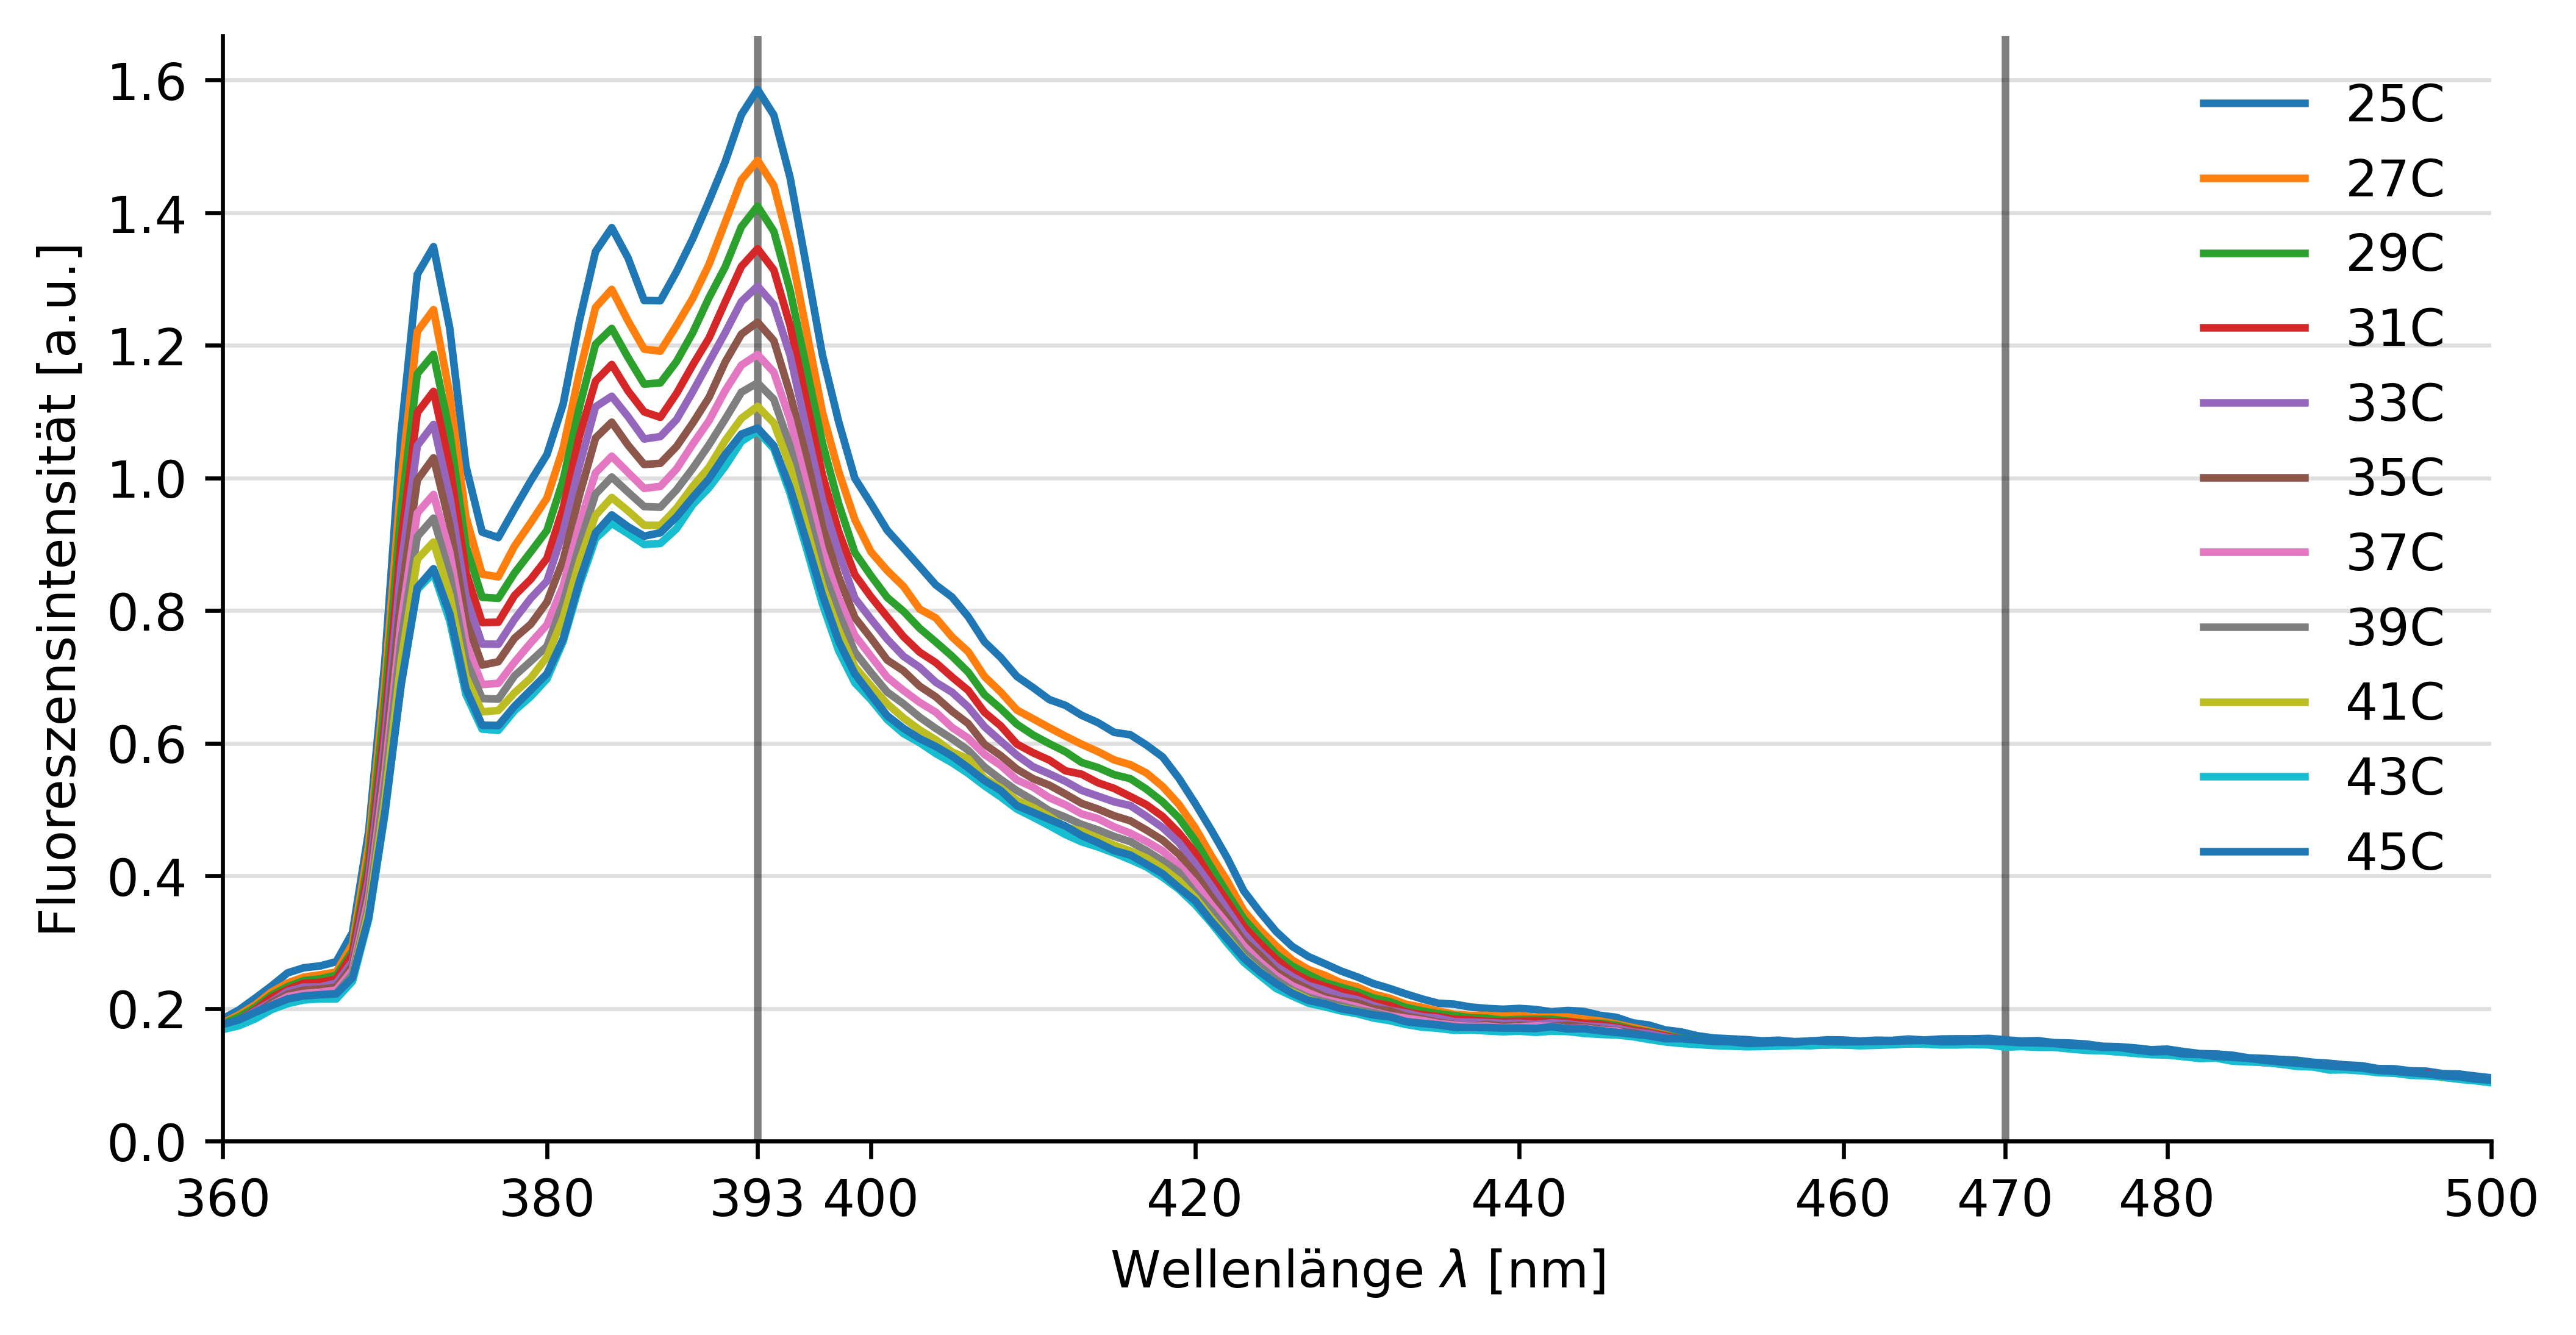
\includegraphics[width=\textwidth]{picture/Temp.png}
			\caption{Fluoreszenzintensität Spektrum von Pyren in Ei-PC; temperaturabhängig} 
			\label{Temp} 
		\end{minipage}
	\end{center}
\end{figure}
Eine Einordnung der errechneten $D_{diff}$ von Pyren (Tabelle \ref{tab:meinetabelle}) in die allgemeine Literatur erweißt sich als schwer, da in keinem Buch beziehungsweise Paper entsprechende Versuche mit $D_{diff}$ Daten gefunden wurden. Die Größenordnung von $D_{diff}$ bezüglich Pyren in Ei-PC stimmt aber annäherend mit ähnlichen Versuchen überein. \cite{Wu1977} \\\\
Das Verhältnis Excimer zu Monomer wird durch die Beweglichkeit und  Konzentrationen bestimmt. \cite{Creuwels1996}\\
Die Fluoreszenzlebenszeiten des Excimers $\tau_0$ (Tab. \ref{tab:Lebenszeiten}) nehmen bei steigender Temperatur wohl deshalb ab, da sich die Diffusionsrate durch Zunahme der Membranfluidität erhöht.\\
Die Technik des Versuchs ist nicht für \textit{flip-flop}  Prozesse geeignet, da der empflindliche Frequenzbereich der Fluoreszenzmessung von circa $10^{-10}\text{ bis } 10^{-7}$ s nicht den Frequenzbereich eines Lipid \textit{flip-flop} Prozess von oft mehr als 1min abdecken kann. \\
Zur Berechnung von $D_{diff}$ bedarf  es Fluoreszenzlebenszeiten $\tau_0$, die durch das Skript gestellt wurden. Unter welchen Bedingungen diese gewonnen wurden, wurde nicht erwähnt. Deshalb sind die in der Tabelle \ref{tab:meinetabelle} dargestellten $D_{diff}$ kritisch zu betrachten. Membranproteine, die sich in realen System befinden, können u.a. ein Hindernis für die Lateraldiffusion $D_{diff}$ von Lipiden darstellen und $D_{diff}$ nahe der Proteine beschränken. Außerdem verändern Proteine die Packungsdichte der Lipide, wodurch kleinere Lipiddomaine entstehen. Die im Versuch gemessenen $D_{diff}$ sind somit eher nur quantitativer Natur. \\
%In Abb. \ref{Ex_Mono} bei DPPC sieht man 2 Übergänge. Einen bei $T=35^\circ C$ und einen bei  $T=43^\circ C$. Der Erste kann ein Artefakt sein bzw. vielleicht kann man darin auch die Ripple Phase $P_{\beta '}$ sehen. Eine engmaschigere Messreihe würde für Klarheit sorgen.\\
%Ei-PC  besitzt gegenüber DPPC (16:0) über ungesättigte Fettsäuren mit cis-Bindungen, die eine Störung der Anordnung der Lipide in der Membran darstellen. Ei-PC verbleibt deswegen im flüssig-kristallinen Zustand $L_\alpha$. DPPC wandelt sich von der Gelphase $L_{\beta '}$ ab circa $T=43^\circ C$ in $L_\alpha$ um, was man indirekt aus der Abb. \ref{Ex_Mono} herauslesen kann. Für eine eindeutige Aussage bezüglich der Phasenumwandlung ist die Technik  des vorliegenden Experiment als alleinstehende Methode weniger geeignet. Die möglichen Phasenumwandlungspunkte für DPPC von $L_{\beta '} \rightarrow P_{\beta '}$ und von $P_{\beta '} \rightarrow L_\alpha$ stimmen aber annäherend mit den Literaturwerten von $36^\circ C$ ($L_{\beta '} \rightarrow P_{\beta '}$) und $41.3^\circ C$ ($P_{\beta '} \rightarrow L_\alpha$) überein \cite{Biltonen1993}.\\
Wichtig festzuhalten ist, dass bei den Messungen im Kapitel \ref{sec:FvonT} nicht exakt bei den angeforderten Temperaturmesspunkten gemessen wurde. Dies liegt im Problem der genauen Einstellbarkeit der Temperatur des Messystem, da die eingestellte Temperatur seltens wirklich erreicht wurde. Deshalb wurde so verfahren, dass, wenn keine Temperaturveränderung nach 2min mehr gemessen wurde, die jeweilige Messung erfollgte, auch wenn bis dahin nicht die eingestelle neue Temperatur erreicht wurde. Dadurch entstand auch ein Fehler, dass nunmehr die Daten nicht zu den angegebenen $\tau_0$ Messwerten aus der Tabelle \ref{tab:Lebenszeiten} passen, wodurch sich die Berechnung von  $D_{diff}$ weiter verfälscht.

%\newpage

	
	\bibliographystyle{siam} 
	\renewcommand{\refname}{Referenzen} 
	\bibliography{Literatur}\newpage
	\section{Anhang}

%Fluoreszenzintensität von DPPC als Funktion der Temperatur 
\begin{figure}[h!]
	\begin{center}
		\begin{minipage}{0,8\textwidth}
			
			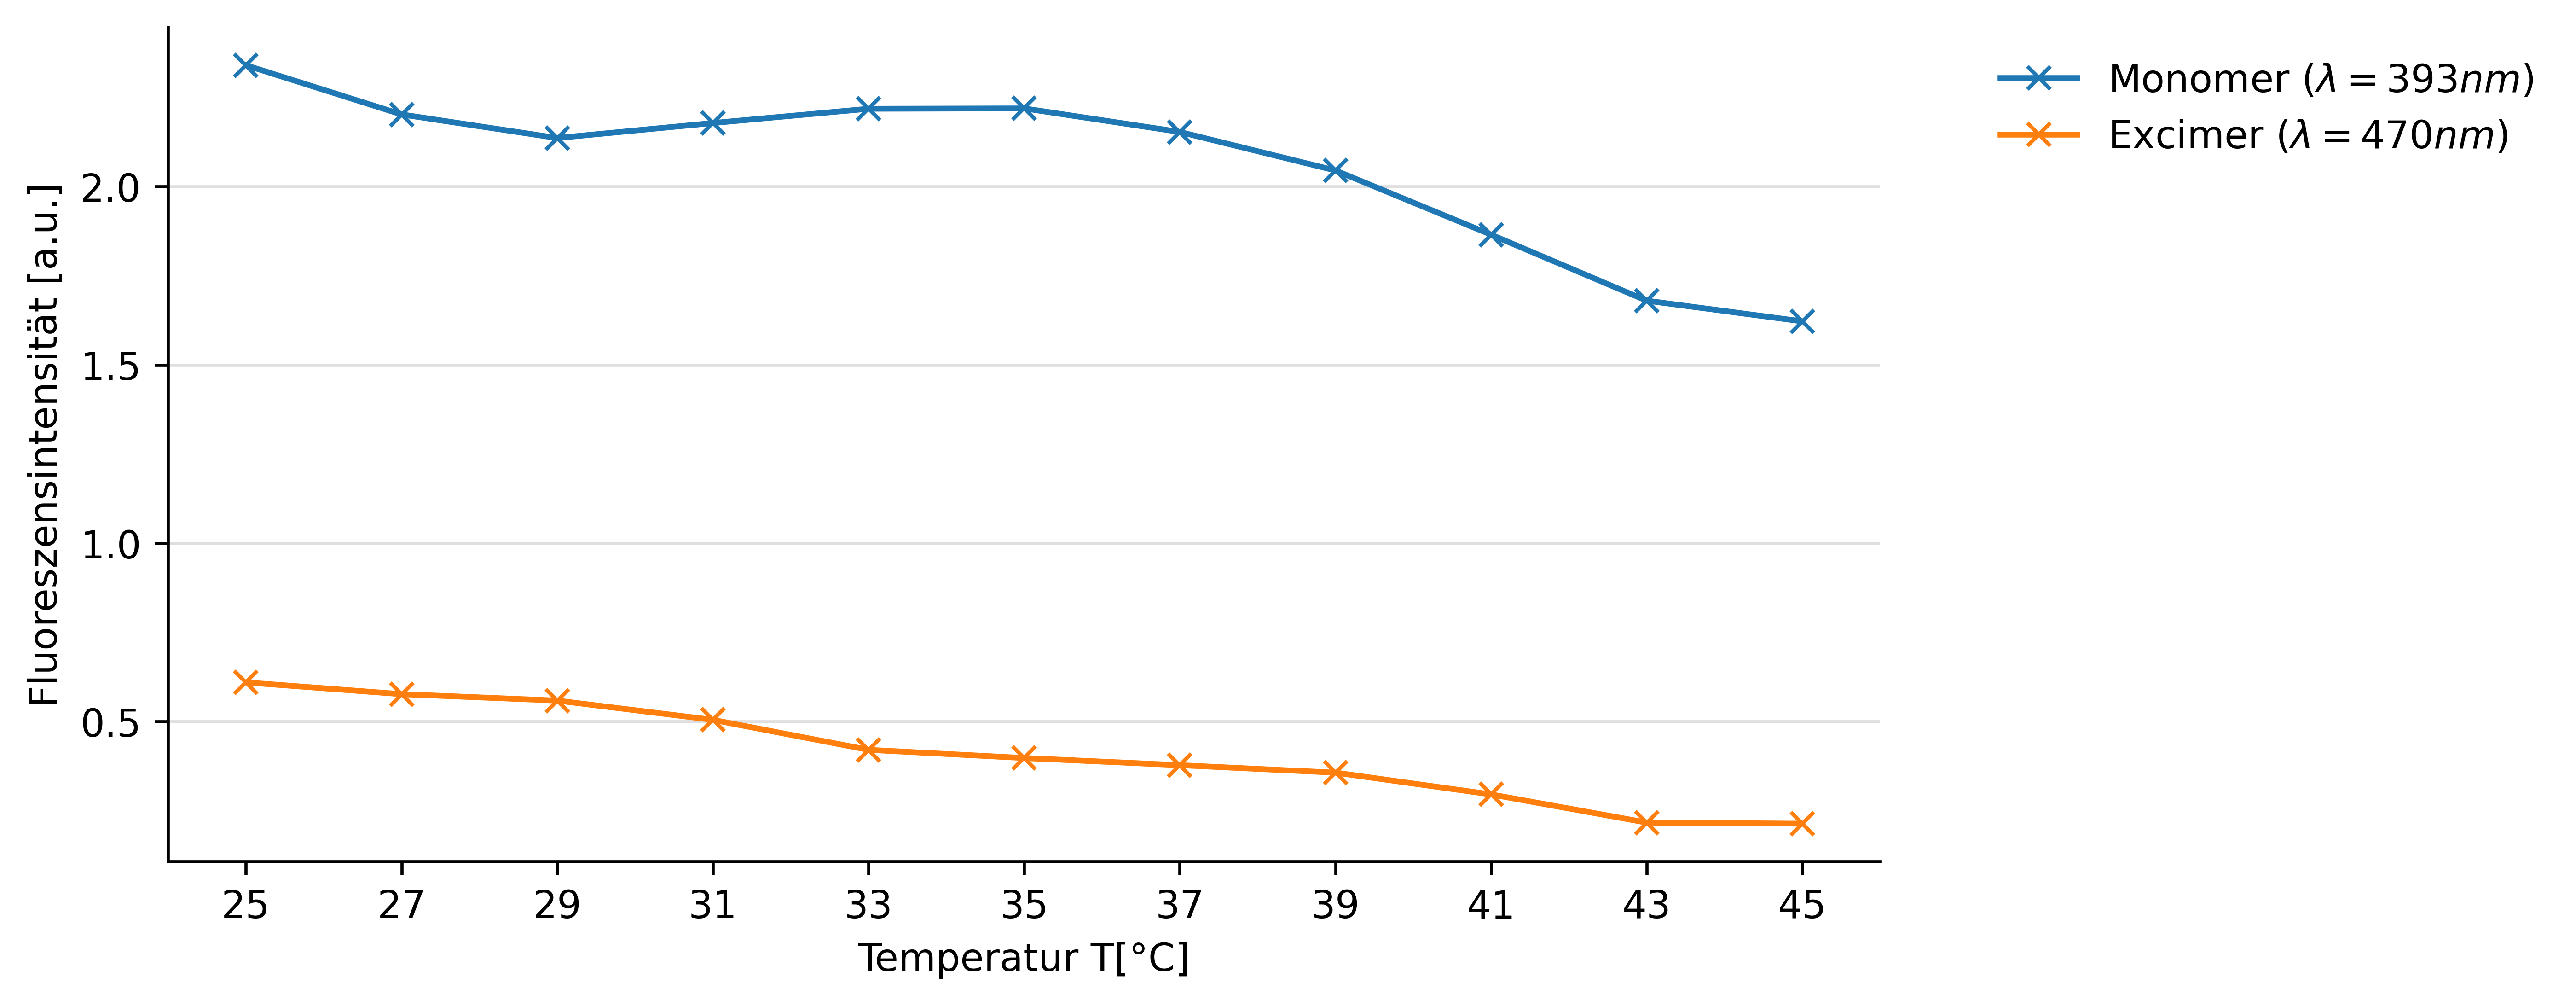
\includegraphics[width=\textwidth]{analysis/reports/DPPC_Temp.png}
			\caption{Pyren in DPPC Vesikeln; Fluoreszenzintensität als Funktion der Temperatur} 
			\label{Monomer_Temp} 
		\end{minipage}
	\end{center}
\end{figure}

%Fluoreszenzintensität von Ei-PC als Funktion der Temperatur 
\begin{figure}[h!]
	\begin{center}
		\begin{minipage}{0,8\textwidth}
			
			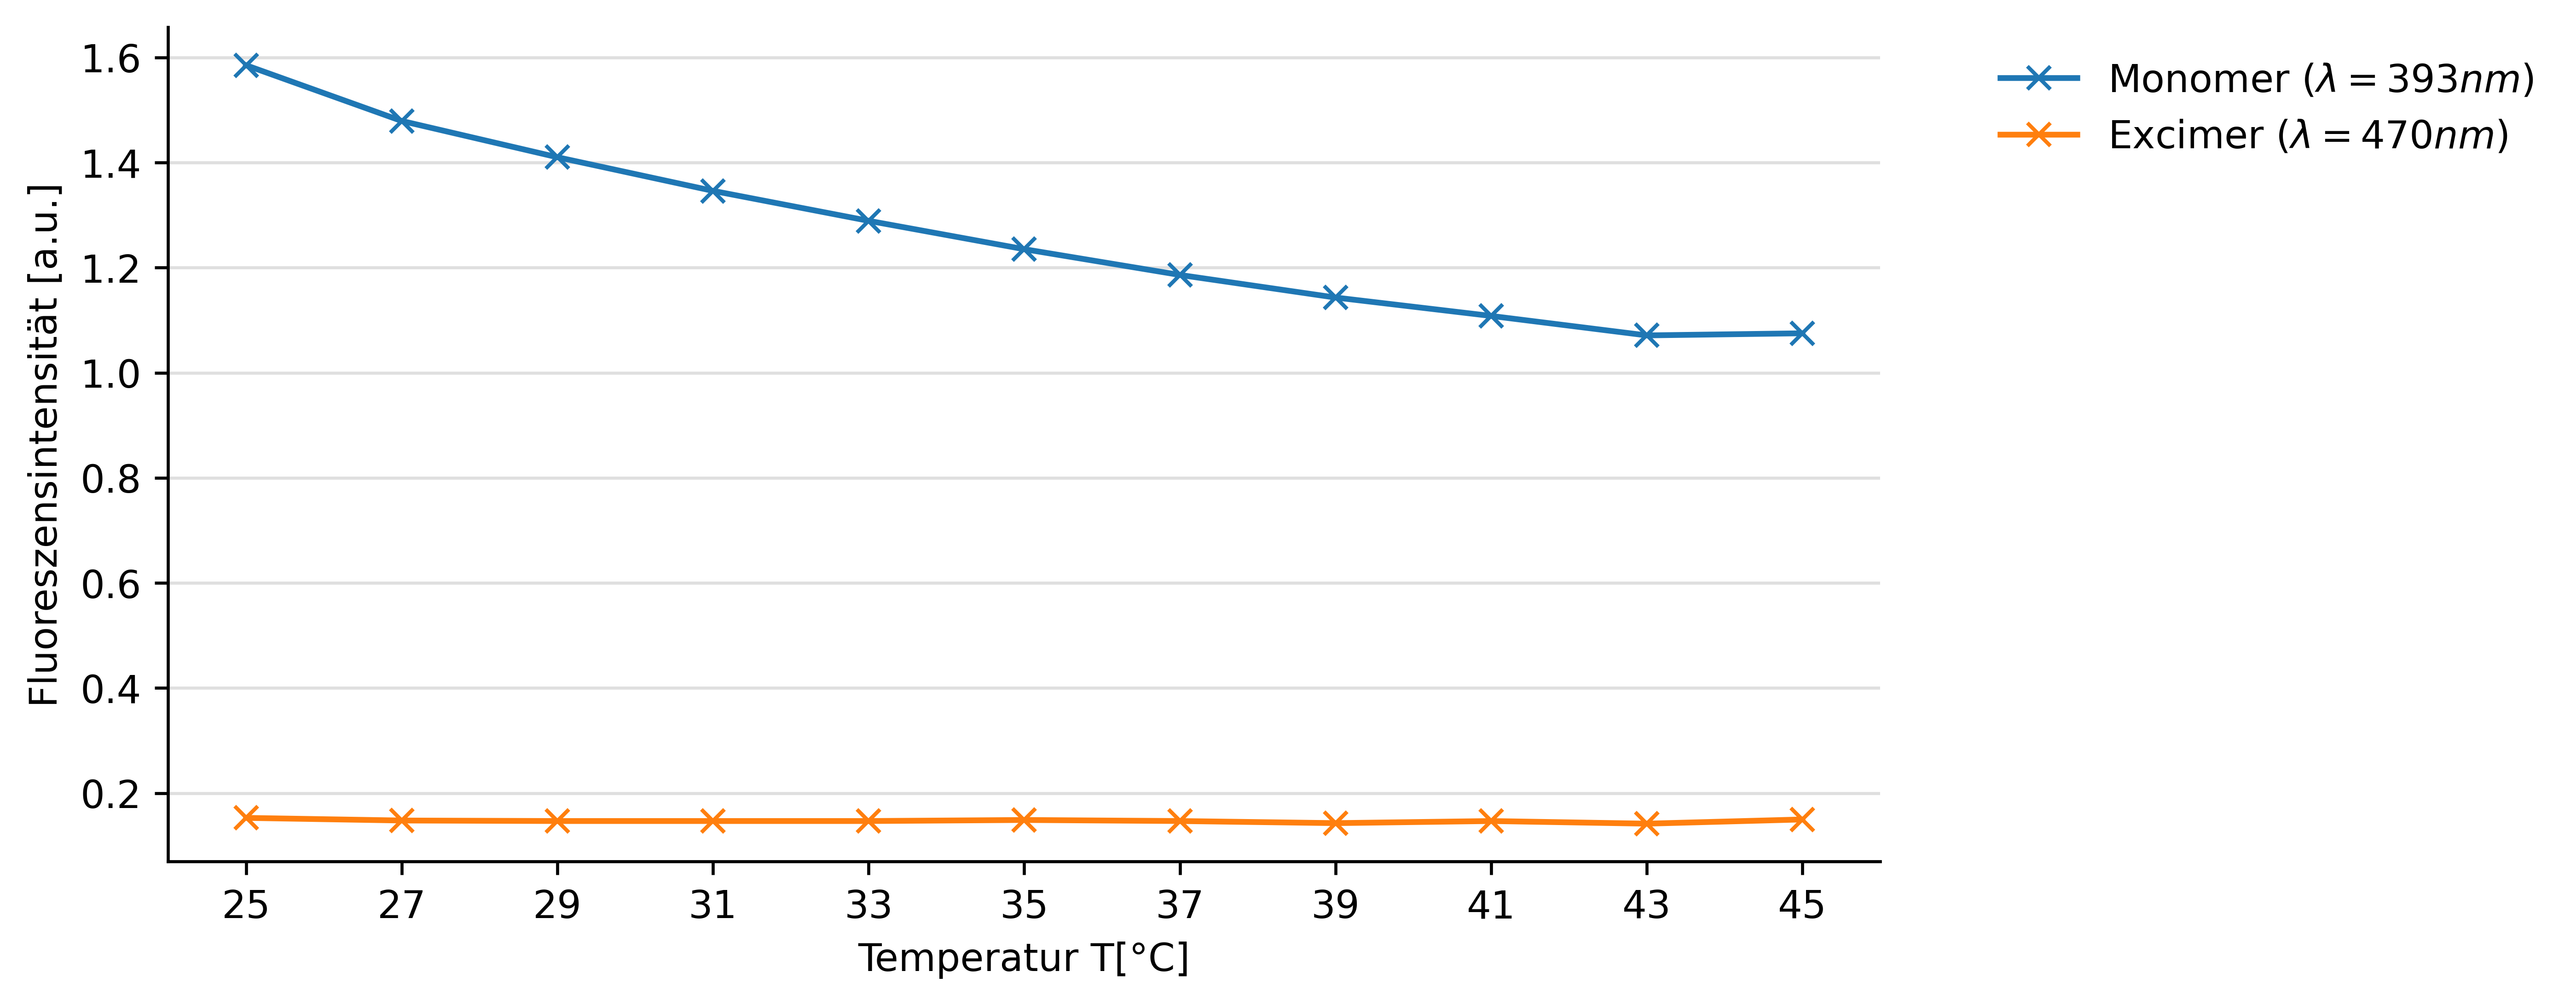
\includegraphics[width=\textwidth]{analysis/reports//Ei-PC_Temp.png}
			\caption{Pyren in Ei-PC Vesikeln; Fluoreszenzintensität als Funktion der Temperatur} 
			\label{Excimer_Temp} 
		\end{minipage}
	\end{center}
\end{figure}





\end{document}